\documentclass[10pt,a4paper]{article}
\usepackage{epsfig,color,colordvi,amsmath,amssymb,listings,cancel,latexsym}
%\usepackage{cancel,amsmath,amssymb,listings,color}
\pagestyle{empty}
\pretolerance=10000
\topmargin=0mm
\headheight=0mm
\headsep=0mm
\textwidth=180mm
\textheight=240mm
\footskip=15mm
\oddsidemargin=-10mm
\evensidemargin=-10mm
\parskip=5mm
\parindent=0mm
\raggedright

\newcommand{\dd}{\partial}
\newcommand{\bk}{\mathbf{k}}
%+CMR
\newcommand{\simlt}{{\raisebox{-1.5mm}{$
\stackrel{\textstyle{<}}{\sim}$}}}
\newcommand{\simgt}{{\raisebox{-1.5mm}{$
\stackrel{\textstyle{>}}{\sim}$}}}
\newcommand{\grad}{{\bfm \nabla}}
\newcommand{\gradv}{{\bfm \nabla_v}}
\newcommand{\dv}[1]{\bfm{ \nabla.{#1}}}
\newcommand{\pd}[2]{\frac{\partial{#1}}{\partial{#2}} }
\newcommand{\curl}[1]{\bfm{\nabla \times {#1}}}
\newcommand{\lapl}{{\bfm \nabla}^{2}}
\newcommand{\und}{\underline}
\newcommand{\half}{\frac{1}{2}}
\newcommand{\abs}[1]{\mid {#1} \mid}
\newcommand{\Z}{{\rm Z}^{\circ}}
\newcommand{\ee}{{\rm e}^{+}{\rm e}^{-}}
\newcommand{\gamgam}{\gamma \gamma}
\newcommand{\tautau}{\tau^{+} \tau^{-}}
\newcommand{\gamgamgam}{\gamma \gamma \gamma}
\newcommand{\bfm}[1]{\mbox{{\boldmath $ { #1}$}}}
\newcommand{\hf}{\frac{1}{2}}
\newcommand{\grads}{{\bfm \nabla_s}}
\newcommand{\gradpar}{\nabla_{\parallel}}
\newcommand{\gradperp}{\bfm{\nabla}_{\perp}}
\newcommand{\ggp}{\nabla_{\parallel}^{\rm GS2}}
\newcommand{\gradeq}{\bfm{\nabla}^{\rm GS2}_{\rm eq}}
\newcommand{\gperp}{\bfm{\nabla}^{\rm GS2}_{\perp}}
\newcommand{\gradl}{{\bfm \nabla_l}}
\renewcommand{\curl}{\bfm{\nabla \times}}
\newcommand{\n}[1]{{#1}_{\rm ref\;}}
\newcommand{\g}[1]{\mathsf{#1}}
\newcommand{\flav}[1]{\left\langle{#1}\right\rangle}
\renewcommand{\Re}[1]{{\rm Re}\left( #1 \right)}
\definecolor{light-gray}{gray}{0.80}
\definecolor{gray}{gray}{0.50}
%-CMR
\title{Final Report for the High Level Support Team DGGS2 Project}
\author{P.\ J.\ Knight$^{1,2}$, C.\ M.\ Roach$^2$, W.\ Arter$^2$ \\
~\\
\small $^1$ EFDA HPC-FF High Level Support Team, CCFE Staff Member\\
\small $^2$ EURATOM/CCFE Fusion Association, Culham Science Centre, Abingdon, OX14
3DB, UK}
\date{June 2012}

\begin{document}
\maketitle

\section*{Abstract}

We present a new, fully-explicit solution method for the GS2 gyrokinetic code.
Presently, GS2 uses an implicit algorithm for the evolution of linear terms,
which is numerically stable for large time-steps in linear simulations.
However, initialising the implicit response matrices is an expensive operation
in computational terms, and in certain cases needs to be repeatedly performed
throughout the course of the run. It was therefore considered that a move to
create a fully explicit solution method would be beneficial.

The new method is a finite-element Discontinuous Galerkin (DG) scheme, using
an adaptive explicit Runge-Kutta time-stepping solver to advance the solution
accurately in an efficient manner.

This report provides a full description of the method as implemented in GS2,
including a detailed derivation of the chosen DG scheme and the necessary
changes that had to be made to the form of the gyrokinetic equation. A summary
of the adaptive Runge-Kutta time advancement method employed is given,
together with an overview of the code modifications that were made.

We conclude with the presentation of results obtained by running GS2 with the
new explicit scheme, and compare these with results obtained from equivalent
runs with the original implicit scheme. We demonstrate that the DG
implementation has been successful, with close agreement between the two
methods being evident. Finally, we discuss possible future enhancements that
would expand the usable set of scenarios that could be modelled with the DG
scheme.

\section{Introduction and Motivation}

GS2 is a time-dependent gyrokinetic code used widely for the simulation of
plasma microinstabilities and turbulence. It uses the gyrokinetic equation to
evolve the 5-D phase space perturbed density distribution function $g_s$:
\begin{align}
\frac{\partial g_s}{\partial t} + (v_\parallel \mathbf{b} +
\mathbf{v}_d).\nabla g_s + C_s \, g_s & = -q_s \frac{\partial f_{0s}}{\partial E}
\frac{\partial \chi}{\partial t} + \left\{ \chi, f_{0s} \right\} \\
\left\{ \chi, f_{0s} \right\} & = \frac{1}{B} \nabla_{\perp} \chi \times
\mathbf{b}.\nabla f_{0s} \nonumber \\
\chi & = (\Phi - v_\parallel \, A_\parallel) J_0(Z) + \frac{m_s \,
v_\perp^2}{q_s} \frac{B_\parallel}{B} \frac{J_1(Z)}{Z} \nonumber \\
\mbox{where} \;\;\;\;\;
Z_s & = k_\perp \rho_s \nonumber
\end{align}
The perturbed electromagnetic fields $\Phi, A_\parallel, B_\parallel$
contributing to the gyrokinetic electromagnetic potential $\chi$ are
determined self-consistently from Maxwell's equations. Full details about the
derivation and implementation of the field equations are contained in the
Appendix.

Presently, GS2 uses an implicit algorithm for the evolution of linear
terms~\cite{kotschenreuther}, which is numerically stable for large time-steps
in linear simulations. However, initialising the implicit response matrices
has a computational cost that scales strongly with grid size along the field
line direction. Such a cost is expensive if the simulation is aimed at
resolving disparate scales, such as
\begin{itemize}
\item microtearing modes
\item multi-scales with both ion temperature gradient (ITG) and electron
  temperature gradient (ETG) modes present
\item for equilibria with low finite magnetic shear.
\end{itemize}
The nonlinear term is handled pseudo-spectrally in space (perpendicular to the
field lines) with an explicit second order Adams-Bashforth time stepping
scheme; thus, in nonlinear simulations the time-step is limited by the CFL
condition. Since changing the time-step requires the code to perform the
expensive re-initialisations of the large response matrix, it was considered
that a move to create a fully explicit solution method would be beneficial.
Our new explicit algorithm will complement the implicit algorithm, and
facilitate larger grid simulations by reducing the large initialisation
overhead.

The DGGS2 project builds on the preceding OPTGS2 and IMPGS2 projects, which
undertook a study of Discontinuous Galerkin (DG) schemes, including both
implicit and explicit schemes, for the 1-D advection equation and the
linearised Vlasov equation. It was found that DG could provide more accurate
solutions than schemes such as MacCormack and PPM~\cite{hammer}.

\section{The Discontinuous Galerkin Scheme}
\label{sec:dgscheme}

In this section we describe the mathematical formulation used to derive the
algorithm coded into GS2. Although based on the discussion in~\cite{hammer} we
provide here a more comprehensive description of the method, and extend it to
include the actual implementation details.

The OPTGS2 project demonstrated the ability of a DG scheme using a finite
element mesh to evolve a standard 1-D advection equation. The gyrokinetic
equation\footnote{Although the distribution function $g$ evolved by GS2 is a
  5-D object, four of the dimensions are `parallelised out', leaving the
  poloidal angle $z$ as the only remaining co-ordinate to consider in this
  discussion.} evolved by GS2 is similar to the 1-D advection equation, and
can be written in a suitable form (see Section~\ref{sec:gkeqn_rearrangment})
that allows us to use the proposed DG scheme as an alternative to the existing
implicit scheme in the code.

\subsection{Derivation for simple advection equation}

We start by considering the simple 1-D advection equation without sources:
\begin{equation}
\frac{\dd g}{\dd t} + v \frac{\dd g}{\dd z} = 0
\label{eqn:basicadvection}
\end{equation}
In GS2 the $z$ direction means the direction parallel to the field lines, or
equivalently the poloidal angle $\theta$.

\subsubsection{Discretisation of the spatial domain}

We divide the domain into a set of $N_e$ finite elements, centred at $z_1, z_2,
\cdots , z_{N_e}$ and represent $g$ on each element $i$ as an approximation $g_i$
obtained by fitting a polynomial of order $(p-1)$ to $g$. Each element
straddles $p$ grid points (`nodes'), which are equally-spaced in $z$ (see
Figure~\ref{fig:elements}).

\begin{figure}[ht]
  \begin{center}
    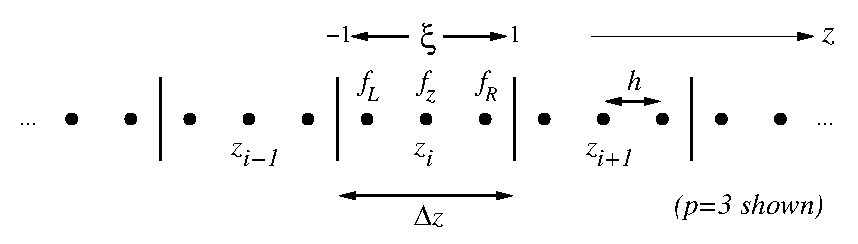
\epsfig{file=finite_elements.eps,width=16cm,angle=0}
  \end{center}
  \caption{\textit{Diagram showing relationship between finite elements
      and nodal grid points.}
    \label{fig:elements} }
\end{figure}

At present the scheme implemented in the code requires that the $N_e$ finite
elements exactly cover the $N_z$ (= \texttt{2*ntgrid + 1}) grid points, i.e.\
$N_z = p\, N_e$. Thus, the extreme ends of the $z$ domain are located at grid
point~1 of element $i=1$ and grid point~$p$ of element $i=N_e$. The reason for
the present implementation is to allow the arrays used for the nodal and modal
representations of a given quantity to be identical in size and shape for
convenience, as $p$ modal coefficients describe the polynomial fit through $p$
grid points.

It is also necessary for symmetry that $z=0$ be a grid point, so this provides
the constraint that $p$ must be odd. Thus our DG implementation assumes that
$p=3$ is a suitable choice.

(Note that the above requirements severely limit the allowed values of GS2
grid dimensioning variables \texttt{nperiod} and \texttt{ntheta}, and
therefore also \texttt{ntgrid}, but this requirement could be relaxed
relatively straightforwardly by modifying the boundary condition treatment
described later.)

% The lowest order DG scheme with one central node gives an upwind scheme
% which is effectively already coded (for advection), so the indicated schemes
% will have $2$ and~$3$~nodes per element. Similarly, only low order
% Runge-Kutta~(RK) schemes are needed for the time advance. Indeed, the task
% should commence with $3$rd~order RK, since $2$nd~order is not expected
% to be adequate to treat the~$i \omega_d$ operator below in Eqn~stst,
% with error control as described by Watts and Shampine, see Sec-control.
% Similarly, to preserve the symmetry of the current finite difference 
% representation, it is necessary to start with $3$-node spatial elements.

We treat each element separately to begin with (hence `discontinuous'), and
fit the polynomial over the local domain, $-1 \leq \xi \leq 1$:
\[
g_i(\xi) = \sum_{m=0}^{p-1} \hat{g}_{i,m} P_m(\xi)
\]
where $P(\xi)$ represents a suitable polynomial form. The objects
$\hat{g}_{i,m}$ are the `modal' coefficients of the polynomial terms used in
the fit.

We solve Equation~\ref{eqn:basicadvection} by asserting that the residual $R_i$ of the
approximation must be orthogonal to any test function $\tau(z)$ in the domain
$z_{i-\frac{1}{2}} \leq z \leq z_{i+\frac{1}{2}}$:
\begin{align}
R_i(z,t) & = \frac{\dd g_i}{\dd t} + v \frac{\dd g_i}{\dd z} \nonumber \\
\int_{{z_{i-\frac{1}{2}}}}^{z_{i+\frac{1}{2}}} \tau(z) \, R_i(z,t) \, dz & =
\int_{{z_{i-\frac{1}{2}}}}^{z_{i+\frac{1}{2}}} \tau \left( \frac{\dd g_i}{\dd t} +
  v \frac{\dd g_i}{\dd z} \right) dz = 0
\label{eqn:residual}
\end{align}
(Henceforth we will represent $z_{i-\frac{1}{2}}$ by $z_-$, and
$z_{i+\frac{1}{2}}$ by $z_+$.)

We integrate the second term of Equation~\ref{eqn:residual} by parts:
\[
\int_{z_-}^{z_+} v \tau \frac{\dd g_i}{\dd z} \, dz = \left[ v \tau g_i
\right]_{z_-}^{z_+} - v \int_{z_-}^{z_+} \frac{\dd \tau}{\dd z} g_i \, dz
\]
So (\ref{eqn:residual}) becomes
\begin{align}
\int_{z_-}^{z_+} \tau(z) \frac{\dd g_i(z)}{\dd t} \, dz - v \int_{z_-}^{z_+}
\frac{\dd \tau(z)}{\dd z} g_i(z) \, dz & = -\left[ v \tau g_i
\right]_{z_-}^{z_+}
\label{eqn:intbyparts} \\
& = \tau(z_-)\left\{ v\,g \right\}(z_-) - \tau(z_+)\left\{ v\,g
\right\}(z_+) \nonumber
\end{align}
The terms in $\{\}$ are the numerical fluxes required at the element
boundaries; these fluxes provide the necessary linkage between adjacent
elements. We will assume the simplest, upwind, case in which information only
propagates in the direction of the flow $v$; thus:
\begin{align*}
\left\{ vg \right\}(z_-) & = \left\{
\begin{array}{lc}
v \, g_{i-1}(z_-) & ; \;\; v \geq 0 \\
v \, g_{i}(z_-) & ; \;\; v < 0
\end{array}
\right. \\
\left\{ vg \right\}(z_+) & = \left\{
\begin{array}{lc}
v \, g_{i}(z_+) & ; \;\; v \geq 0 \\
v \, g_{i+1}(z_+) & ; \;\; v < 0
\end{array}
\right.
\end{align*}

\subsubsection{Change of spatial co-ordinate variable}
\label{sec:spatialvarchange}

Let us now make the change of variable from $z$ to $\xi$ (see
Figure~\ref{fig:elements}):
\begin{align*}
\xi & = -1 \;\;\; \mbox{at} \;\;\; z = z_{i-\frac{1}{2}} = z_- \\
\xi & = +1 \;\;\; \mbox{at} \;\;\; z = z_{i+\frac{1}{2}} = z_+ \\
\mbox{By inspection,} \;\;\; \xi(z) & = \frac{2(z-z_i)}{z_+ - z_-} \\
& = \frac{2z - 2 \left(\frac{z_+ + z_-}{2}\right)}{z_+ - z_-} \\
\Longrightarrow \;\;\; \xi(z) & = \frac{2z - (z_+ + z_-)}{z_+ - z_-} \\
\frac{d\xi}{dz} & = \frac{2}{z_+ - z_-} = \frac{2}{\Delta z}
\end{align*}
where $\Delta z$ is the spatial extent covered by the finite element; $\Delta
z = h\,p$, with $h$ being the separation of the nodal points on the original
grid.

Observe that, for $p=3$, the three nodes within each element are at $\xi =
-\frac{2}{3}$, $\xi = 0$, and $\xi = \frac{2}{3}$.

\subsubsection{Legendre polynomials as base functions}

We now choose a suitable basis for our fitting polynomial $P(\xi)$ and test
function $\tau$. The Legendre polynomials provide one such set of base
functions, and have the following properties:
\begin{align*}
& P_0(x) = 1 \;\;\; , \;\;\; P_1(x) = x \;\;\;\;\;\; (-1 \leq x \leq 1) \\
\mbox{Recurrence formula:} \;\;\; & P_n(x) = \frac{2n-1}{n} x \, P_{n-1}(x) -
\frac{n-1}{n} P_{n-2}(x) \\
\mbox{Orthogonality:} \;\;\; \int_{-1}^{1} & P_n(x) \, P_m(x) \, dx =
\frac{2}{2n+1} \, \delta_{nm}
\end{align*}
where $\delta_{nm}$ is the Kronecker delta.

A smooth function $g(z)$ can be expanded as a series of Legendre polynomials:
\[
g(z) = \sum_{m=0}^\infty \hat{g}_m P_m(z)
\]
and the coefficients $\hat{g}_m$ are obtained via the relation
\[
\hat{g}_m = \frac{2m+1}{2} \int_{-1}^{1} g(z) \, P_m(z) \, dz
\]
Thus the LHS of Equation~\ref{eqn:intbyparts} may be written as follows; we
replace $\tau(z)$ by $P_n(\xi)$, and $g_i(z)$ by $\sum_{m=0}^{p-1} \hat{g}_{i,m}
P_m(\xi)$, so
\[
\mbox{LHS} = \int_{z_-}^{z_+} \tau(z) \frac{\dd g_i(z)}{\dd t} \, dz - v \int_{z_-}^{z_+}
\frac{\dd \tau(z)}{\dd z} g_i(z) \, dz
\]
becomes
\[
\mbox{LHS} = \int_{-1}^{1} P_n(\xi) \sum_{m=0}^{p-1} P_m(\xi) \frac{d\hat{g}_{i,m}}{dt}
\, \frac{dz}{d\xi} \, d\xi - v \int_{-1}^{1} \frac{dP_n(\xi)}{dz}
\sum_{m=0}^{p-1} P_m(\xi) \, \hat{g}_{i,m} \frac{dz}{d\xi} \, d\xi
\]
and the RHS terms involving the numerical fluxes become:
\begin{align*}
\tau(z_-) \left\{ vg \right\}(z_-) & = \left\{
\begin{array}{lc}
v \, P_n(-1) \sum_{m=0}^{p-1} \, \hat{g}_{i-1,m} \, P_m(1) & ; \;\; v \geq 0 \\
v \, P_n(-1) \sum_{m=0}^{p-1} \, \hat{g}_{i,m} \, P_m(-1) & ; \;\; v < 0
\end{array}
\right. \\
\tau(z_+) \left\{ vg \right\}(z_+) & = \left\{
\begin{array}{lc}
v \, P_n(1) \sum_{m=0}^{p-1} \, \hat{g}_{i,m} \, P_m(1) & ; \;\; v \geq 0 \\
v \, P_n(1) \sum_{m=0}^{p-1} \, \hat{g}_{i+1,m} \, P_m(-1) & ; \;\; v < 0
\end{array}
\right.
\end{align*}
So, Equation~\ref{eqn:intbyparts} becomes 
\begin{align}
\sum_{m=0}^{p-1} \left\{ \frac{dz}{d\xi} \left( \int_{-1}^{1} P_n(\xi)
  \, P_m(\xi) \, d\xi \right) \frac{d\hat{g}_{i,m}}{dt} \right\} {}&
- v \sum_{m=0}^{p-1} \left\{ \frac{dz}{d\xi} \left( \int_{-1}^{1}
    \frac{dP_n(\xi)}{dz} P_m(\xi) \, d\xi \right) \hat{g}_{i,m} \right\}
\nonumber \\
& = \left\{
\begin{array}{lc}
v \, P_n(-1) \sum_{m=0}^{p-1} P_m(1) \, \hat{g}_{i-1,m} -
v \, P_n(1) \sum_{m=0}^{p-1} P_m(1) \, \hat{g}_{i,m} & ; \;\; v \geq 0 \\
v \, P_n(-1) \sum_{m=0}^{p-1} P_m(-1) \, \hat{g}_{i,m} - 
v \, P_n(1) \sum_{m=0}^{p-1} P_m(-1) \, \hat{g}_{i+1,m} & ; \;\; v < 0
\end{array}
\right.
\label{eqn:legendred} 
\end{align}

\subsubsection{Mass, stiffness and flux matrices}

We can simplify the LHS of Equation~\ref{eqn:legendred} by introducing the `mass
matrix' $M_{nm}$ and the `stiffness matrix' $D_{nm}$, as follows:
\begin{align*}
M_{nm} & \equiv \frac{dz}{d\xi} \int_{-1}^{1} P_n(\xi) \, P_m(\xi) \, d\xi \\
D_{nm} & \equiv \frac{dz}{d\xi} \int_{-1}^{1} \frac{dP_n(\xi)}{dz} \, P_m(\xi) \, d\xi
\end{align*}
The LHS of Equation~\ref{eqn:legendred} becomes simply
\[
\mbox{LHS} = \sum_{m=0}^{p-1} M_{nm} \, \frac{d\hat{g}_{i,m}}{dt} - v \sum_{m=0}^{p-1}
D_{nm} \, \hat{g}_{i,m}
\]
We also introduce four flux matrices $F_{nm}$ to simplify the RHS
of Equation~\ref{eqn:legendred}:
\begin{align*}
F_{nm}^{i-1,v_+} & \equiv P_n(-1) \, P_m(1) \\
F_{nm}^{i,v_+} & \equiv P_n(1) \, P_m(1) \\
F_{nm}^{i,v_-} & \equiv P_n(-1) \, P_m(-1) \\
F_{nm}^{i+1,v_-} & \equiv P_n(1) \, P_m(-1)
\end{align*}
\begin{align*}
\Longrightarrow \;\;\;
v \, P_n(-1) \sum_{m=0}^{p-1} P_m(1) \, \hat{g}_{i-1,m} & = v \, F^{i-1,v_+} \,
\hat{\mathbf{g}}_{i-1} \\
v \, P_n(1) \sum_{m=0}^{p-1} P_m(1) \, \hat{g}_{i,m} & = v \, F^{i,v_+} \,
\hat{\mathbf{g}}_{i} \\
v \, P_n(-1) \sum_{m=0}^{p-1} P_m(-1) \, \hat{g}_{i,m} & = v \, F^{i,v_-} \,
\hat{\mathbf{g}}_{i} \\
v \, P_n(1) \sum_{m=0}^{p-1} P_m(-1) \, \hat{g}_{i+1,m} & = v \, F^{i+1,v_-} \,
\hat{\mathbf{g}}_{i+1}
\end{align*}
where $\hat{\mathbf{g}}_j$ denotes the column vector of length $p$ containing
the values $\hat{g}_{j,0}, \hat{g}_{j,1}, \cdots, \hat{g}_{j,p-1}$ for element $j$.

So we have, for $v \geq 0$,
\begin{align}
\sum_{m=0}^{p-1} M_{nm} \frac{d\hat{g}_{i,m}}{dt} & = v \left[
  \sum_{m=0}^{p-1} D_{nm} \, \hat{g}_{i,m} + \sum_{m=0}^{p-1} F_{nm}^{i-1,v_+} \,
  \hat{g}_{i-1,m} - \sum_{m=0}^{p-1} F_{nm}^{i,v_+} \, \hat{g}_{i,m} \right] \nonumber \\
 & = v \left[
  \sum_{m=0}^{p-1} F_{nm}^{i-1,v_+}  \, \hat{g}_{i-1,m} + \sum_{m=0}^{p-1}
  \left(D_{nm} - F_{nm}^{i,v_+}\right) \hat{g}_{i,m} \right]
\label{eqn:sumvplus}
\end{align}
and for $v < 0$,
\begin{align}
\sum_{m=0}^{p-1} M_{nm} \frac{d\hat{g}_{i,m}}{dt} & = v \left[
  \sum_{m=0}^{p-1} D_{nm} \, \hat{g}_{i,m} + \sum_{m=0}^{p-1} F_{nm}^{i,v_-} \,
  \hat{g}_{i,m} - \sum_{m=0}^{p-1} F_{nm}^{i+1,v_-} \, \hat{g}_{i+1,m} \right] \nonumber \\
 & = v \left[
  \sum_{m=0}^{p-1} \left(D_{nm} + F_{nm}^{i,v_- }\right) \hat{g}_{i,m} -
  \sum_{m=0}^{p-1} F_{nm}^{i+1,v_-} \, \hat{g}_{i+1,m} \right]
\label{eqn:sumvminus}
\end{align}

We now evaluate the matrices $M_{nm}$, $D_{nm}$, $F_{nm}$ using the properties
of Legendre polynomials.

The mass matrix is
\begin{align*}
M_{nm} & \equiv \frac{dz}{d\xi} \int_{-1}^{1} P_n(\xi) \, P_m(\xi) \, d\xi \\
& = \frac{\Delta z}{2} \frac{2}{2n+1} \delta_{nm}
\end{align*}
\[
\Longrightarrow \;\;\; \boxed{ M_{nm}  = \frac{\Delta z}{2n+1} \delta_{nm} }
\]
In matrix form\footnote{Reminder: $n$ denotes row number starting from zero,
  while $m$ denotes column number starting from zero.}, for $p=3$
\begin{align*}
M & = \Delta z \left(
\begin{array}{ccc}
1 & 0 & 0 \\
0 & \frac{1}{3} & 0 \\
0 & 0 & \frac{1}{5}
\end{array} \right) \\
\Longrightarrow \;\;\; M^{-1} & = \frac{1}{\Delta z} \left(
\begin{array}{ccc}
1 & 0 & 0 \\
0 & 3 & 0 \\
0 & 0 & 5
\end{array} \right)
\end{align*}

To evaluate the stiffness matrix $D_{nm}$ we use the following recurrence
relation involving the derivatives of Legendre polynomials:
\begin{align*}
(2m+1) P_m(x) & = \frac{dP_{m+1}(x)}{dx} - \frac{dP_{m-1}(x)}{dx} \\
\Longrightarrow \;\;\; \frac{dP_{m+1}(x)}{dx} & = (2m+1) P_m(x) +
\frac{dP_{m-1}(x)}{dx} \\
\mbox{Relabelling: $n=m+1$} \Longrightarrow \;\;\; \frac{dP_n(x)}{dx} & =
\left( 2(n-1)+1 \right) P_{n-1}(x) +
\frac{dP_{n-2}(x)}{dx} \\
& = \left(2(n-1)+1\right) P_{n-1}(x) + \left(2(n-3)+1\right) P_{n-3}(x) +
\cdots
\end{align*}
This can be written as the following series:
\newcommand{\oddsum}
{ \sum_{
\mbox{\scriptsize{ $\begin{array}{c} j=0 \\ j+n \mbox{ odd} \end{array}$ }}
}^{n-1} }
\[
\frac{dP_n(x)}{dx} =
\oddsum (2j+1) \, P_j(x)
\]
The criterion `$j+n \equiv $ odd' is required, since if $n$ is odd, the only
non-zero terms are for $j=n-1,n-3,\cdots,0$, i.e.\ $j$ is even. Similarly, if
$n$ is even, the only non-zero terms are for $j=n-1,n-3,\cdots,1$, i.e.\ $j$
is odd.

So, $D$ is evaluated as follows:
\begin{align*}
D_{nm} & \equiv \frac{dz}{d\xi} \int_{-1}^{1} \frac{dP_n(\xi)}{dz} \, P_m(\xi)
\, d\xi \\
& = \frac{dz}{d\xi} \int_{-1}^{1} \frac{d\xi}{dz} \frac{dP_n(\xi)}{d\xi} \, P_m(\xi)
\, d\xi \\
& = \int_{-1}^{1} \frac{dP_n(\xi)}{d\xi} \, P_m(\xi) \, d\xi \\
& = \int_{-1}^{1} \oddsum (2j+1) \, P_j(\xi) \, P_m(\xi) \, d\xi \\
& = \oddsum (2j+1) \int_{-1}^{1} P_j(\xi) \, P_m(\xi) \, d\xi \\
& = \oddsum (2j+1) \frac{2}{2j+1} \delta_{jm}
\end{align*}
\[
\Longrightarrow \;\;\; \boxed{ D_{nm} = \oddsum 2 \, \delta_{jm} }
\]
In matrix form, for $p=3$
\[
D = \left( \begin{array}{ccc}
0 & 0 & 0 \\
1 & 0 & 0 \\
0 & 1 & 0
\end{array} \right)
\left( \begin{array}{ccc}
2 & 0 & 0 \\
0 & 2 & 0 \\
0 & 0 & 2
\end{array} \right)
\]
The first matrix encodes the logic $[\mbox{column } j] \leq ([\mbox{row } n]-1)$
\texttt{AND} $(j+n)$ is odd. The second matrix is simply $2 \delta_{jn}$.
\[
\Longrightarrow \;\;\; D = \left( \begin{array}{ccc}
0 & 0 & 0 \\
2 & 0 & 0 \\
0 & 2 & 0
\end{array} \right)
\]

Finally, the flux matrices are easily calculated using the identities
\begin{align*}
P_n(1) & = 1 \;\;\; \mbox{for all $n$} \\
P_n(-1) & = (-1)^n \\
P_n(-1) \, P_m(-1) & = (-1)^n (-1)^m = (-1)^{n+m}
\end{align*}
So, for $p=3$
\begin{align*}
F^{i-1,v_+} = \left( \begin{array}{rrr}
1 & 1 & 1 \\
-1 & -1 & -1 \\
1 & 1 & 1
\end{array} \right) & , \;\;\;
F^{i,v_+} = \left( \begin{array}{rrr}
1 & 1 & 1 \\
1 & 1 & 1 \\
1 & 1 & 1
\end{array} \right) \\
F^{i,v_-} = \left( \begin{array}{rrr}
1 & -1 & 1 \\
-1 & 1 & -1 \\
1 & -1 & 1
\end{array} \right) & , \;\;\;
F^{i+1,v_-} = \left( \begin{array}{rrr}
1 & -1 & 1 \\
1 & -1 & 1 \\
1 & -1 & 1
\end{array} \right) \\
\end{align*}

So, at last we can write down in matrix form the equations relevant to $v \geq
0$ and $v < 0$. Equation~\ref{eqn:sumvplus} for $v \geq 0$ is
\begin{align*}
\sum_{m=0}^{p-1} M_{nm} \frac{d\hat{g}_{i,m}}{dt} & = v \left[
  \sum_{m=0}^{p-1} F_{nm}^{i-1,v_+}  \, \hat{g}_{i-1,m} + \sum_{m=0}^{p-1}
  \left(D_{nm} - F_{nm}^{i,v_+}\right) \hat{g}_{i,m} \right] \\
\Longrightarrow \;\;\;
\frac{d\hat{\mathbf{g}}_{i}}{dt} & = v \, M^{-1} \left( F^{i-1,v_+}
  \hat{\mathbf{g}}_{i-1} + \left(D - F^{i,v_+}\right)\hat{\mathbf{g}}_{i} \right)
\end{align*}
or, explicitly,
\begin{equation}
\frac{d}{dt} \left( \begin{array}{c}
\hat{g}_{i,0} \\ \hat{g}_{i,1} \\ \hat{g}_{i,2}
\end{array} \right)
=
\frac{v}{\Delta z} \left(
\begin{array}{ccc}
1 & 0 & 0 \\
0 & 3 & 0 \\
0 & 0 & 5
\end{array} \right)
\left(
\begin{array}{rrrrrr}
1 & 1 & 1 & -1 & -1 & -1 \\
-1 & -1 & -1 & 1 & -1 & -1 \\
1 & 1 & 1 & -1 & 1 & -1 \\
\end{array} \right)
\left( \begin{array}{c}
\hat{g}_{i-1,0} \\ \hat{g}_{i-1,1} \\ \hat{g}_{i-1,2} \\
\hat{g}_{i,0} \\ \hat{g}_{i,1} \\ \hat{g}_{i,2}
\end{array} \right)
 \;\;\;\;\;\; v \geq 0
\label{eqn:fullmatrixeqnvplus}
\end{equation}

Similarly, Equation~\ref{eqn:sumvminus} for $v < 0$ is
\begin{align*}
\sum_{m=0}^{p-1} M_{nm} \frac{d\hat{g}_{i,m}}{dt} & = v \left[
  \sum_{m=0}^{p-1} \left(D_{nm} + F_{nm}^{i,v_-}\right) \hat{g}_{i,m}
- \sum_{m=0}^{p-1} F_{nm}^{i+1,v_-}  \, \hat{g}_{i+1,m}
  \right] \\
\Longrightarrow \;\;\;
\frac{d\hat{\mathbf{g}}_{i}}{dt} & = v \, M^{-1} \left(
  \left(D + F^{i,v_-}\right)\hat{\mathbf{g}}_{i}
- F^{i+1,v_-} \hat{\mathbf{g}}_{i+1} \right)
\end{align*}
or, explicitly,
\begin{equation}
\frac{d}{dt} \left( \begin{array}{c}
\hat{g}_{i,0} \\ \hat{g}_{i,1} \\ \hat{g}_{i,2}
\end{array} \right)
=
\frac{v}{\Delta z} \left(
\begin{array}{ccc}
1 & 0 & 0 \\
0 & 3 & 0 \\
0 & 0 & 5
\end{array} \right)
\left(
\begin{array}{rrrrrr}
1 & -1 & 1 & -1 & 1 & -1 \\
1 & 1 & -1 & -1 & 1 & -1 \\
1 & 1 & 1 & -1 & 1 & -1 \\
\end{array} \right)
\left( \begin{array}{c}
\hat{g}_{i,0} \\ \hat{g}_{i,1} \\ \hat{g}_{i,2} \\
\hat{g}_{i+1,0} \\ \hat{g}_{i+1,1} \\ \hat{g}_{i+1,2}
\end{array} \right)
 \;\;\;\;\;\; v < 0
\label{eqn:fullmatrixeqnvminus}
\end{equation}

\subsection{Modifications for actual advection equation form in GS2}
\label{sec:mods}

Recall that the above derivation was for the simplest form of the advection
equation~(\ref{eqn:basicadvection}). However, the form of the equation in GS2
is more complicated:
\begin{equation}
  \frac{\dd g}{\dd t} + i \, \omega_d \, g + v_\parallel \frac{\dd}{\dd z} (g+\mathcal{F})
  = S
\label{eqn:gs2form4dg}
\end{equation}
These variations are translated into the matrix equations, as follows: \footnotesize
\begin{equation} \boxed{
\frac{d}{dt} \left( \begin{array}{c}
\hat{g}_{i,0} \\ \hat{g}_{i,1} \\ \hat{g}_{i,2}
\end{array} \right)
=
-i \left( \begin{array}{c}
\widehat{\omega_d\,g}_{i,0} \\ \widehat{\omega_d\,g}_{i,1} \\ \widehat{\omega_d\,g}_{i,2}
\end{array} \right)
+ \frac{v_\parallel}{\Delta z} \left(
\begin{array}{ccc}
1 & 0 & 0 \\
0 & 3 & 0 \\
0 & 0 & 5
\end{array} \right)
\left(
\begin{array}{rrrrrr}
1 & 1 & 1 & -1 & -1 & -1 \\
-1 & -1 & -1 & 1 & -1 & -1 \\
1 & 1 & 1 & -1 & 1 & -1 \\
\end{array} \right)
\left( \begin{array}{c}
\hat{g}_{i-1,0} + \hat{\mathcal{F}}_{i-1,0} \\
\hat{g}_{i-1,1} + \hat{\mathcal{F}}_{i-1,1} \\
\hat{g}_{i-1,2} + \hat{\mathcal{F}}_{i-1,2} \\
\hat{g}_{i,0} + \hat{\mathcal{F}}_{i,0} \\
\hat{g}_{i,1} + \hat{\mathcal{F}}_{i,1} \\
\hat{g}_{i,2} + \hat{\mathcal{F}}_{i,2}
\end{array} \right)
+ \left( \begin{array}{c}
\hat{S}_{i,0} \\ \hat{S}_{i,1} \\ \hat{S}_{i,2}
\end{array} \right)
} \;\;\;\;\;\; v_\parallel \geq 0
\label{eqn:vplus}
\end{equation}
\begin{equation} \boxed{
\frac{d}{dt} \left( \begin{array}{c}
\hat{g}_{i,0} \\ \hat{g}_{i,1} \\ \hat{g}_{i,2}
\end{array} \right)
=
-i \left( \begin{array}{c}
\widehat{\omega_d\,g}_{i,0} \\ \widehat{\omega_d\,g}_{i,1} \\ \widehat{\omega_d\,g}_{i,2}
\end{array} \right)
+ \frac{v_\parallel}{\Delta z} \left(
\begin{array}{ccc}
1 & 0 & 0 \\
0 & 3 & 0 \\
0 & 0 & 5
\end{array} \right)
\left(
\begin{array}{rrrrrr}
1 & -1 & 1 & -1 & 1 & -1 \\
1 & 1 & -1 & -1 & 1 & -1 \\
1 & 1 & 1 & -1 & 1 & -1 \\
\end{array} \right)
\left( \begin{array}{c}
\hat{g}_{i,0} + \hat{\mathcal{F}}_{i,0} \\
\hat{g}_{i,1} + \hat{\mathcal{F}}_{i,1} \\
\hat{g}_{i,2} + \hat{\mathcal{F}}_{i,2} \\
\hat{g}_{i+1,0} + \hat{\mathcal{F}}_{i+1,0} \\
\hat{g}_{i+1,1} + \hat{\mathcal{F}}_{i+1,1} \\
\hat{g}_{i+1,2} + \hat{\mathcal{F}}_{i+1,2}
\end{array} \right)
+ \left( \begin{array}{c}
\hat{S}_{i,0} \\ \hat{S}_{i,1} \\ \hat{S}_{i,2}
\end{array} \right)
} \;\;\;\;\;\; v_\parallel < 0
\label{eqn:vminus}
\end{equation} 
\normalsize
(In the above, non-subscripts $i = \sqrt{-1}$, while subscripts containing $i$
continue to refer to elements, as before.)

Note that there is the slight complication in that $\omega_d$ and
$v_\parallel$ are not independent of $z$, so it is important to take the
product of such terms with $g$ etc.\ in `nodal' space before converting the
result to modal form.  We have shown this above for the $i \,
(\widehat{\omega_d \, g})_{i,m}$ terms, but the same approach must be used for
the $v_\parallel \, \dd(g+\mathcal{F})/\dd z$ terms.

\subsection{Conversion between nodal and modal forms}

During the evaluation of Equations~\ref{eqn:vplus} and~\ref{eqn:vminus}, and
also elsewhere in the solution process, it is necessary to be able to convert
back and forth between modal and nodal representations. Recall that in the
$p=3$ scheme, each finite element spans three equally-spaced grid points in
the $z$ direction. Within each element we fit Legendre polynomials $P_n(\xi)$,
$n=0,1,2$, over the internal range $\xi=(-1,1)$ through the three grid points,
which lie at $\xi=-\frac{2}{3}$, $\xi=0$, $\xi=\frac{2}{3}$, respectively. For
some quantity $f$, we can label its values at the three points as $f_L$, $f_z$
and $f_R$ respectively, and we can find the corresponding modal coefficients
$\hat{f}_0,\hat{f}_1,\hat{f}_2$ by solving the three equations stemming from
the following definition:
\[
f(\xi) = \hat{f}_0\,P_0(\xi) + \hat{f}_1\,P_1(\xi) + \hat{f}_2\,P_2(\xi)
\]
i.e.
\begin{align*}
f_L & = \hat{f}_0\,P_0\left(-\frac{2}{3}\right) +
\hat{f}_1\,P_1\left(-\frac{2}{3}\right) + \hat{f}_2\,P_2\left(-\frac{2}{3}\right) \\ 
f_z & = \hat{f}_0\,P_0\left(0\right) + \hat{f}_1\,P_1\left(0\right) +
\hat{f}_2\,P_2\left(0\right) \\
f_R & = \hat{f}_0\,P_0\left(\frac{2}{3}\right) + \hat{f}_1\,P_1\left(\frac{2}{3}\right) +
\hat{f}_2\,P_2\left(\frac{2}{3}\right)
\end{align*}
where the Legendre polynomials are defined as
\begin{align*}
P_0(\xi) & = 1 \\
P_1(\xi) & = \xi \\
P_2(\xi) & = \frac{1}{2} (3 \xi^2 - 1)
\end{align*}
Thus, to convert from nodal values to modal coefficients, we have
\begin{align*}
f_L & = \hat{f}_0 - \frac{2}{3}\,\hat{f}_1 + \frac{1}{6}\,\hat{f}_2 \\
f_z & = \hat{f}_0 - \frac{1}{2}\,\hat{f}_2 \\
f_R & = \hat{f}_0 + \frac{2}{3}\,\hat{f}_1 + \frac{1}{6}\,\hat{f}_2 \\
\mbox{or} \;\;\; \left( \begin{array}{c}
f_L \\ f_z \\ f_R
\end{array} \right)
& = \left( \begin{array}{rrr}
\rule{0pt}{4mm} 1 & -\frac{2}{3} & \frac{1}{6} \\
\rule{0pt}{4mm} 1 & 0 & -\frac{1}{2} \\
\rule{0pt}{4mm} 1 & \frac{2}{3} & \frac{1}{6}
\end{array} \right)
\left( \begin{array}{c}
\hat{f}_0 \\ \hat{f}_1 \\ \hat{f}_2
\end{array} \right)
\end{align*}
and to make the reverse transformation we have the following relationship (by
matrix inversion):
\begin{align*}
\left( \begin{array}{c}
\hat{f}_0 \\ \hat{f}_1 \\ \hat{f}_2
\end{array} \right)
& = \left( \begin{array}{rrr}
\rule{0pt}{4mm} \frac{3}{8} & \frac{1}{4} & \frac{3}{8} \\
\rule{0pt}{4mm} -\frac{3}{4} & 0 & \frac{3}{4} \\
\rule{0pt}{4mm} \frac{3}{4} & -\frac{3}{2} & \frac{3}{4}
\end{array} \right)
\left( \begin{array}{c}
f_L \\ f_z \\ f_R
\end{array} \right)
\end{align*}

\section{Solution procedure and boundary conditions}
\label{sec:solution}

The procedure for evaluating $d\hat{g}/dt$ and dealing with the boundary
conditions is performed in routine \texttt{dgdt\_dggs2}, and may be summarised
as follows:
\begin{enumerate}

\item The input to the routine is the array of coefficients comprising
  $\hat{g}$ for all the finite elements, where $\hat{g}$ represents the modal
  coefficients for a \textit{fully-consistent}\/ (i.e.\ boundary condition
  satisfying) distribution function $g$; either the quantity from the previous
  time-step ($g_{\mbox{\scriptsize old}}$), or an intermediate $g$ calculated
  at a particular step in the Runge-Kutta algorithm (see
  Section~\ref{sec:rk}).

\item $\hat{g}$ is converted to its nodal representation $g$, and this is used
  to calculate the physical quantities $\Phi$, $A_\parallel$, $B_\parallel$ by
  evaluating the Maxwell field equations; see later Sections for more
  details. These are then used to calculate the source term $S$ and the flux
  function $\mathcal{F}$ at each grid point. $S$ is converted to its modal
  form $\hat{S}$.

\item The $-i\, \omega_d \,g$ term is calculated at each grid point, and
  converted to its modal representation.

\item The quantity $g+\mathcal{F}$ is calculated and converted to modal form,
  and the relevant matrix multiplication is done to perform the $d/dz$
  operation as described above (in particular, in Section~\ref{sec:mods}). The
  result is converted back to nodal form to enable the multiplication by
  $v_\parallel/\Delta z$ to be done correctly (remembering the definition of
  $\Delta z$ from Section~\ref{sec:spatialvarchange}), after which the product
  is returned to modal form.

  Note that Equation~\ref{eqn:vplus} for $v_\parallel \geq 0$ uses values from
  element $i-1$, i.e.\ the one to the left of the current element $i$, to
  calculate the $d/dz$ terms, and Equation~\ref{eqn:vminus} for $v_\parallel <
  0$ uses values from element $i+1$. At the extreme ends of the domain, this
  is dealt with by conceptually adding a `ghost' element to the left or right
  as appropriate, containing zeroes for coefficients. This ensures that the
  $d/dz$ terms are not contaminated with spurious contributions from outside
  the true domain.

\item At this point we now have all the terms on the RHS of
  Equations~\ref{eqn:vplus} and~\ref{eqn:vminus} in modal form, which we
  simply sum to obtain the $d\hat{g}/dt$ array.

\item We can now apply the necessary boundary conditions \textit{a
    posteriori}. It must be remembered that this is an \textit{explicit}\/
  scheme. As long as the \textit{input}\/ $\hat{g}$ array is consistent with
  the boundary conditions (which it should be!), the nodal $dg/dt$ values
  corresponding to the just-calculated $d\hat{g}/dt$ coefficients are
  guaranteed to be correct at all grid points, except (possibly) at those grid
  points at which the boundary conditions must be re-applied. Unlike in the
  existing implicit algorithm, no integration is performed in the $z$
  direction---we are evaluating $dg/dt$, not $g$, and the $d/dz$ terms are
  evaluated explicitly via the matrix equations. We may therefore safely apply
  the boundary conditions at the required points \textit{a posteriori},
  without affecting the $dg/dt$ values elsewhere.

\end{enumerate}

Passing particles and trapped particles (which occur under certain conditions
at particular pitch angles) have different boundary conditions, and must be
treated separately.

\subsection{Passing particles}

Boundary conditions are applied at the ends of the $z$ domain. The required
constraint is that $g = 0$ for incoming particles, i.e.
\begin{align*}
g(v_\parallel \geq 0) & = 0 \;\;\; \mbox{at the left-most grid point} \\
g(v_\parallel < 0) & = 0 \;\;\; \mbox{at the right-most grid point}
\end{align*}
This is straightforward to implement. We simply convert the $d\hat{g}/dt$
coefficients into nodal form, and set $dg/dt=0$ at the left-most grid point
for the particles with $v_\parallel \geq 0$, and similarly at the right-most
grid point for the particles with $v_\parallel < 0$. Thus, we guarantee that
$g_{\mbox{\scriptsize new}} = g_{\mbox{\scriptsize old}} = 0$ as required.

\subsection{Trapped particles}

Trapped particles exist only within certain portions of the poloidal angle
range; so-called forbidden regions are therefore present for these particles
centred on the inboard side of the flux surface ($\theta = \pm \pi$).
\begin{itemize}

\item The pitch angle $\lambda$ of a field line determines whether there will
  be trapped particles gyrating along it. The logical array
  \texttt{forbid(ig,il)} denotes whether a particular location \texttt{ig} on
  a field line with pitch angle \texttt{il} is within a forbidden region. The
  distribution function $g$ is zero by definition in such regions, so we force
  $dg/dt = 0$ wherever \texttt{forbid(ig,il)} is true.

\item The grid point adjacent to either end of a forbidden region is a
  so-called bounce point, where a trapped particle's parallel velocity
  $v_\parallel$ becomes zero (physically, the particle reverses direction). At
  these points, $g(v > 0) = g(v < 0)$, that is to say, there are as many
  ``right-going'' particles as ``left-going'' particles. Thus we must have
  $dg/dt(v > 0) = dg/dt(v < 0)$ at the bounce points.

\end{itemize}

\textit{Because of ongoing difficulties with the implementation of the bounce point
criteria, it is not yet possible to simulate trapped particles within the DG
scheme. We hope to resolve this situation post-project after additional
discussions with other CCFE researchers on where the problems arise.}

\section{Runge-Kutta Time Advancement}
\label{sec:rk}

The previous Section derived the matrix equations~\ref{eqn:vplus}
and~\ref{eqn:vminus} used to evaluate the rate of change of the $\hat{g}$
coefficients within each finite element with respect to time. To evolve
$\hat{g}$ as accurately as possible we use a Runge-Kutta (RK) scheme to
perform the time-advancement from $\hat{g}_{\mbox{\scriptsize old}}$ to
$\hat{g}_{\mbox{\scriptsize new}}$, and if we use a so-called adaptive RK
scheme we can ensure that the time-step $\Delta t$ used is the most efficient
possible whilst retaining the desired level of accuracy in the solution.

\subsection{Adaptive Runge-Kutta scheme}
\label{sec:rkf}

An explicit RK method may be summarised as follows. The derivative $y^\prime$
of quantity $y$ with respect to (say) time $t$ is evaluated at a number of
test points in the $(y,t)$ plane, and these $y^\prime$ values are combined in
a way specific to the particular RK method in use, to form an estimate of the
new value $y_{n+1}$:
\begin{align*}
y^\prime & = f(t,y) \;\;\; ; \;\;\; y(t_0) = y_0 \\
y_{n+1} & = y_n + \Delta t \sum_{i=1}^s b_i \, k_i
\end{align*}
where
\begin{align*}
k_1 & = f(t_n, y_n) \\
k_2 & = f(t_n + c_2\,\Delta t, y_n + a_{21}\,\Delta t\,k_1) \\
k_3 & = f(t_n + c_3\,\Delta t, y_n + a_{31}\,\Delta t\,k_1 + a_{32}\,\Delta t\,k_2) \\
& \vdots \\
k_s & = f(t_n + c_s\,\Delta t, y_n + a_{s1}\,\Delta t\,k_1 + a_{s2}\,\Delta t\,k_2 + \ldots +
a_{s,s-1}\,\Delta t\,k_{s-1})
\end{align*}
The number of steps $s$ used in a particular method is related to (but not
necessarily the same as) the order $P$ of the scheme. The coefficients used in
the above process may be summarised in a Butcher tableau~\cite{butcher}:
\[
\begin{array}{c|ccccc}
\rule{0pt}{4mm} 0 & & & & & \\
\rule{0pt}{4mm} c_2 & a_{21} & & & & \\
\rule{0pt}{4mm} c_3 & a_{31} & a_{32} & & & \\
\rule{0pt}{4mm} \vdots & \vdots & \vdots & \ddots & & \\
\rule{0pt}{4mm} c_s & a_{s1} & a_{s2} & \ldots & a_{s,s-1} & 0 \\ \hline
\rule{0pt}{4mm} & b_1 & b_2 & \ldots & b_{s-1} & b_s
\end{array}
\]

An adaptive RK scheme uses two methods, typically one of order $P$ and one of
order $P-1$. For efficiency many of the computation steps need not be
replicated as the coefficients are reused in both methods; however, a second
row of $b$ coefficients is added to the Butcher tableau to incorporate the
second method. By computing two estimates for $y_{n+1}$, we obtain an estimate
of the error in the answer by taking the difference between the two, and this
difference is of order $(\Delta t)^{P}$ (this is therefore described as a
$P$th order adaptive scheme). This allows us to adjust the time-step
automatically, given a chosen error tolerance level, to maintain both
sufficient accuracy and efficiency.

The third-order ($P=3$) adaptive scheme we have chosen to use is described by
Stoer and Bulirsch~\cite{stoer_bulirsch}, and has the following Butcher
tableau:
\begin{equation}
\begin{array}{c|cccc}
\rule{0pt}{4mm} 0 & & & & \\
\rule{0pt}{4mm} 0 & \frac{1}{4} & & & \\
\rule{0pt}{4mm} 0 & -\frac{189}{400} & \frac{729}{800} & & \\
\rule[-2mm]{0pt}{6mm} 0 & \frac{214}{891} & \frac{1}{33} & \frac{650}{891} & \\ \hline
\rule{0pt}{4mm}  & \frac{214}{891} & \frac{1}{33} & \frac{650}{891} & 0 \\
\rule{0pt}{4mm}  & \frac{533}{2106} & 0 & \frac{800}{1053} & -\frac{1}{78} \\
\end{array}
\end{equation}
In source file \texttt{fields\_explicit.f90}, we have written a new Fortran~90
module \texttt{rk\_schemes} and a general RK solver routine
\texttt{rk\_advance}, in which the above adaptive scheme is
implemented. Routine \texttt{dgdt\_dggs2} (see Section~\ref{sec:solution})
performs the necessary calculation of $y^\prime = f(t,y)$ as necessary, but
uses as inputs the modal coefficients $\hat{g}$ of the distribution function
to evaluate two estimates for $d\hat{g}/dt$. Hence, \texttt{rk\_advance}
advances the modal coefficients of $g$, rather than $g$ itself.

On exit from \texttt{rk\_advance}, the modal to nodal conversion of the two
estimates of $\hat{g}_{\mbox{\scriptsize new}}$ is performed.

\subsection{Adaptive time-step control}
\label{sec:control}

The time-step control for the above RK pair is based on that used in
subroutine \texttt{rkf45}~\cite{rkf45}, a code for a Fehlberg 4th-5th order RK
method. Time-step control is a potentially difficult area, because of the need
not only to keep errors under control, but to do so efficiently, without
excessively repeating steps. \texttt{rkf45} allows a user to set both a
relative error tolerance and an absolute error level. The treatment for a
general scheme of order~$P$ has been deduced from the original \texttt{rkf45}
code (in which $P=5$).

The principle behind the algorithm may be summarised as follows:
\begin{itemize}

\item We obtain two arrays of values for the updated distribution function
  $g_{\mbox{\scriptsize new}}$ using the adaptive RK method described above,
  namely $g_{\mbox{\scriptsize new},1}$ from the $(P-1)$th order RK advance,
  and $g_{\mbox{\scriptsize new},2}$ from the $P$th order RK advance.

\item The user specifies maximum allowable absolute and relative error
  tolerances between $g_{\mbox{\scriptsize new},1}$ and $g_{\mbox{\scriptsize
      new},2}$, and from these the code computes the ratio $R$ between the
  actual maximum difference $|| g_{\mbox{\scriptsize new},1} -
  g_{\mbox{\scriptsize new},2}||$ and the maximum allowed difference. This
  ensures that the time-step will respond to the most sensitive part of $g$ as
  measured by the difference in the two estimates obtained.

\item The time-step $\Delta t$ to be used on the next time-advance is
  determined by a factor dependent on the value of $R$ and the order of the
  scheme $P$:
\[
\Delta t_{n+1} = \Delta t_n \frac{f}{R^{\frac{1}{P}}}
\]
where $f = 0.9$ is typically used. So, if $R > f^P$ the time-step is reduced
on the next advance, but if $R < f^P$ it is increased, as the algorithm
detects that a larger time-step is tolerable --- see
Figure~\ref{fig:adaptivedt1}. Therefore, under approximately steady-state
conditions the time-step should automatically converge on a value $f^P$ times
the maximum tolerable time-step, or $\Delta t \longrightarrow 0.729\,\Delta
t_{\mbox{\scriptsize max}}$ for $f=0.9, \;\; P=3$.

(The method includes other tests to improve its robustness, not elaborated
upon here; for instance if $R > 1$ the code rejects the time-advance that has
just occurred, and does the advance again but with the new, lower $\Delta t$.)

\end{itemize}

\begin{figure}[!p]
  \begin{center}
    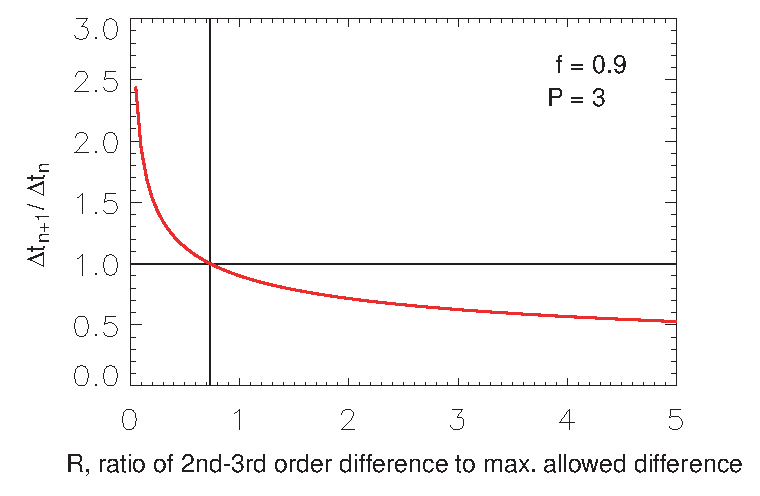
\epsfig{file=adaptivedt1.eps,width=16cm,angle=0}
  \end{center}
  \caption{\textit{Plot showing how the time-step varies according to the
      accuracy achieved on the previous iteration. In a well-behaved scenario,
      the time-step will settle down on a value such that $R=f^P$, indicated
      by the crossing-point shown.}
    \label{fig:adaptivedt1} }
\end{figure}

% The time-step control for the above RK pair is based on that used in
% subroutine \texttt{rkf45} from \texttt{netlib}, a code for a Fehlberg
% fourth-fifth order Runge-Kutta method written by H.\ A.\ Watts and L.\ F.\
% Shampine. Time-Step control is a potentially difficult area, because of the
% need not only to keep errors under control, but to do so efficiently, without
% excessively repeating steps. \texttt{rkf45} allows a user to set both a
% relative error tolerance~$\epsilon_r$, and an absolute error
% level~$\epsilon_a$, where it is recommended that $\epsilon_r > 10^{-12}$.  The
% treatment for a general scheme of order~$p$, where $p=5$ for \texttt{rkf45},
% has been deduced from Watts and Shampine's code.  It is convenient to define
% also variables $r_\epsilon=2/\epsilon_r$ and $\epsilon_{ar}=2
% \epsilon_a/\epsilon_r$. The treatment of the first step is different from that
% of subsequent steps, so the two are treated separately below.

% Initially, set~$g$ and calculate~$\dot{g}$ at time $t=0$. The former is used
% to calculate the total allowed error as
% \begin{equation}
% \epsilon_t= \epsilon_r || g || + \epsilon_a
% \end{equation}
% where $|| \cdot ||$ denotes a norm of~$g$, and \texttt{rkf45} uses the maximum
% norm~$L_{\infty}$.
% Supposing the user suggests an initial time-step of~$\Delta t_0$, then this
% will be used as $\Delta t$ for the first step unless
% \begin{equation}
% \Delta t_e = \left(\frac{\epsilon_t}{||\dot{g}||}\right)^\frac{1}{p}
% \end{equation}
% is smaller, or $\epsilon_{ro}\Delta t_0$ is larger, where $\epsilon_{ro}$ is a 
% quantity
% one to two orders of magnitude larger than the machine 
% epsilon~$\epsilon_{mach}$.
% In the exceptional cases just described, the alternative value of time-step
% is used instead of~$\Delta t_0$.

% In subsequent steps, suppose that provisionally $\bar{g}$ and $\hat{g}$ have
% been calculated at time~$t+\Delta t$, then the key parameter which decides
% whether $\Delta t$ allows the error tolerances to be satisfied is
% \begin{equation}
% R_s= r_\epsilon \Delta t \left( \frac{|| \hat{g}-\bar{g} ||}{||\hat{g}|| + 
% ||g^n|| + \epsilon_{ar}} \right)
% \end{equation}
% where $g^n$ is the value of~$g$ at time~$t$ calculated using the last
% acceptable (previous) time-step. Note that Watts and Shampine are careful
% to calculate $|| \hat{g}-\bar{g} ||$ to minimise rounding error,
% using the difference in the increments of $g$, rather than 
% differences of~$\hat{g}$ and~$\bar{g}$ themselves, which may mean that
% a larger~$\epsilon_{ro}$ is needed when this trick cannot be used.
% It will be seen that $R_s \leq 1$ corresponds to an acceptably small
% value of error as measured by the difference in results
% obtained using the $(p-1)^{th}$ and $p^{th}$~order Runge-Kutta schemes,
% and so $g^{n+1}=\hat{g}$. However, the algorithm then goes onto test 
% whether a larger time-step $h_f \Delta t$ might produce acceptable results in
% subsequent time advances, where $h_f \leq 5$,
% a numerical value apparently chosen on the
% basis of experience as leading to efficient control, together with
% the parameter $\epsilon_1 = 0.1$. The test is whether $R_s > R_c$, where
% \begin{equation}\label{eq:rc}
% R_c = \left( \frac{1-\epsilon_1}{h_{f0}} \right)^p
% \end{equation}
% where~$h_{f0}=5$, and then
% \begin{equation}\label{eq:hf}
% h_f = \frac{1-\epsilon_1}{R_s^{1/p}}
% \end{equation}
% is used provided it is less than~$5$, unless the previous value of $R_s$ was 
% too large, in which
% case $h_f=1$ to prevent a potentially infinite loop of adjustments to $\Delta 
% t$. 

% If the quantity~$R_s > 1$, then the time-step~$\Delta t$ was too large
% and must be reduced to $h_f \Delta t$, 
% where $h_f \geq 0.1$,
% a numerical value again apparently chosen on the
% basis of experience as leading to efficient control. In this case
% the test is as to whether $R_s < R_c$ where $R_c$ is defined in Eqn-rc
% with~$h_{f0}=0.1$,
% and then Eqn-hf is used to determine the new~$h_f\geq0.1$. A flag is set to
% indicate failure at step size~$\Delta t$ and the time-step is repeated
% with size~$h_f \Delta t$ (unless this would be smaller than the
% minimum allowed time-step~$\epsilon_{ro} \Delta t_0$,
% in which case the time advance is terminated completely).

\section{The GS2 Gyrokinetic Equation and DG}
\label{sec:gkeqn_rearrangment}

We turn now to the physics, and describe how we rearrange the gyrokinetic
equation so that it is in a suitable form for the DG implementation.

\subsection{Rearrangement of the form of the GS2 gyrokinetic equation}

The non-adiabatic part of the perturbed distribution function $g_s$ is obtained
from the linearised electromagnetic gyrokinetic equation:
\begin{align}
  \frac{\dd g_s}{\dd t} + (v_\parallel \mathbf{b} + \mathbf{v_d}).\nabla g_s +
  C_s g_s & = -q_s \frac{\dd f_{0s}}{\dd E} \frac{\dd \chi}{\dd t} + 
  \left\{ \chi, f_{0s}\right\} \label{eqn:g}\\
  \mbox{where} \;\;\; \chi & = \left(\Phi - v_\parallel A_\parallel \right)
  J_0(Z) + \frac{m_s v_\perp^2}{q_s} \frac{B_\parallel}{B}
  \frac{J_1(Z)}{Z} \label{eqn:chi} \\
  \mbox{and} \;\;\; \left\{ \chi, f_{0s}\right\} & = \frac{1}{B} \nabla_\perp
  \chi \times \mathbf{b}.\nabla f_{0s}
\end{align}
GS2 solves the gyrokinetic equation above for a modified form of the perturbed
distribution function $h_s$:
\begin{equation}
  h_s = g_s - \frac{q_s}{T_s} \Phi J_0(Z) f_{0s} - \frac{m_s v_\perp^2}{T_s}
  \frac{B_\parallel}{B} \frac{J_1(Z)}{Z} f_{0s}
\label{eqn:h}
\end{equation}
It should be noted that GS2 confusingly uses the variable named \texttt{g} for
$g_s$ \textbf{and}\/ $h_s$ (though of course never both at the same time);
conversion between the two is performed via subroutine \texttt{g\_adjust}.

Combining Equations~\ref{eqn:g}, \ref{eqn:chi} and \ref{eqn:h} gives the form of the
gyrokinetic equation that is numerically solved in GS2:
\begin{align}
  \frac{\dd h_s}{\dd t} + (v_\parallel \mathbf{b} + \mathbf{v_d}).\nabla h_s +
  C_s g_s & = q_s v_\parallel J_0(Z) \frac{\dd f_{0s}}{\dd E} \frac{\dd
    A_\parallel}{\dd t} \nonumber \\
  {}& - f_{0s}(v_\parallel \mathbf{b} + \mathbf{v_d}).\nabla 
  \left[ \frac{q_s}{T_s} \Phi J_0(Z) +\frac{m_s v_\perp^2}{T_s}
    \frac{B_\parallel}{B} \frac{J_1(Z)}{Z} \right] + \left\{ \chi,
    f_{0s}\right\} 
  \label{eqn:h_evolution}
\end{align}
The right hand side of Equation~\ref{eqn:h_evolution} is evaluated by routine
\texttt{set\_source}, `\texttt{contain}'ed within routine \texttt{get\_source\_term} in
\texttt{dist\_fn.f90}.

In order to convert this equation into a form suitable for use with the DG
scheme discussed later, it is necessary to subsume the $\dd A_\parallel / \dd
t$ term into the left hand side, and this may be done by introducing another
change of variables:
\begin{align}
  i_s & = h_s + \frac{q_s}{T_s} v_\parallel A_\parallel J_0(Z) f_{0s}
  \label{eqn:h2i} \\
  & = g_s - \frac{q_s}{T_s}  \chi f_{0s}
\end{align}
The conversion between $h_s$ and $i_s$ is performed via new subroutine
\texttt{g\_adjust\_exp} in source file \texttt{dist\_fn.f90}.

Equation~\ref{eqn:h_evolution} becomes
\begin{align}
  \frac{\dd i_s}{\dd t} + (v_\parallel \mathbf{b} + \mathbf{v_d}).\nabla i_s
  & - \frac{\dd}{\dd t} \left( \frac{q_s}{T_s} v_\parallel A_\parallel J_0(Z)
    f_{0s} \right) - (v_\parallel \mathbf{b} + \mathbf{v_d}).\nabla \left(
    \frac{q_s}{T_s} v_\parallel A_\parallel J_0(Z) f_{0s} \right)
  + C_s g_s \nonumber \\
  = {}& q_s v_\parallel J_0(Z) \frac{\dd f_{0s}}{\dd E} \frac{\dd
    A_\parallel}{\dd t} 
  - f_{0s}(v_\parallel \mathbf{b} + \mathbf{v_d}).\nabla 
  \left[ \frac{q_s}{T_s} \Phi J_0(Z) +\frac{m_s v_\perp^2}{T_s}
    \frac{B_\parallel}{B} \frac{J_1(Z)}{Z} \right] + \left\{ \chi,
    f_{0s}\right\} \nonumber \\
  \frac{\dd i_s}{\dd t} + (v_\parallel \mathbf{b} + \mathbf{v_d}).\nabla i_s + C_s g_s 
  = {}& q_s v_\parallel J_0(Z) \frac{\dd f_{0s}}{\dd E} \frac{\dd
    A_\parallel}{\dd t} + \frac{\dd}{\dd t} \left( \frac{q_s}{T_s} v_\parallel
    A_\parallel J_0(Z) f_{0s} \right) \nonumber \\
  {}& - f_{0s}(v_\parallel \mathbf{b} + \mathbf{v_d}).\nabla 
  \left[ \frac{q_s}{T_s} \Phi J_0(Z) +\frac{m_s v_\perp^2}{T_s}
    \frac{B_\parallel}{B} \frac{J_1(Z)}{Z} \right] \nonumber \\
  {}& + f_{0s} (v_\parallel \mathbf{b} + \mathbf{v_d}).\nabla \left(
    \frac{q_s}{T_s} v_\parallel A_\parallel J_0(Z) \right)
  + \left\{ \chi, f_{0s}\right\} \nonumber \\
  \frac{\dd i_s}{\dd t} + (v_\parallel \mathbf{b} + \mathbf{v_d}).\nabla i_s + C_s g_s 
  = {}& q_s v_\parallel J_0(Z) \frac{\dd A_\parallel}{\dd t}
  \cancelto{0}{ \left( \frac{\dd f_{0s}}{\dd E} + \frac{f_{0s}}{T_s} \right) }
  \nonumber \\
  {}& - \frac{q_s}{T_s} f_{0s} (v_\parallel \mathbf{b} + \mathbf{v_d}).\nabla
  \left( \Phi J_0(Z) + \frac{m_s v_\perp^2}{q_s} \frac{B_\parallel}{B}
    \frac{J_1(Z)}{Z} - v_\parallel A_\parallel J_0(Z) \right) + \left\{ \chi, f_{0s}\right\}
\end{align}
where the cancellation is due to the properties of the Maxwellian.

This is simplified using Equation~\ref{eqn:chi} to give the following
evolution equation for $i_s$:
\begin{align}
  \frac{\dd i_s}{\dd t} + (v_\parallel \mathbf{b} + \mathbf{v_d}).\nabla i_s +
  C_s g_s & = - \frac{q_s}{T_s} f_{0s} (v_\parallel \mathbf{b} +
  \mathbf{v_d}).\nabla \chi + \left\{ \chi, f_{0s}\right\}
  \nonumber \\
  \Longrightarrow \frac{\dd i_s}{\dd t} + \mathbf{v_d}.\nabla i_s + v_\parallel
  \mathbf{b}.\nabla \left(i_s + \frac{q_s}{T_s} \chi f_{0s} \right) + C_s g_s
  & = - \frac{q_s}{T_s} f_{0s} \mathbf{v_d}.\nabla \chi + \left\{ \chi, f_{0s}\right\}
  \label{eqn:i_evolution} 
\end{align}
Finally, we note the following equivalences:
\[
\mathbf{v_d}.\nabla  \equiv i \omega_d \;\;\; ; \;\;\;
\mathbf{b}.\nabla \equiv \frac{\dd}{\dd z}
\]
and substituting these into Equation~\ref{eqn:i_evolution} we get
\begin{equation}
\boxed{
  \frac{\dd i_s}{\dd t} + i\,\omega_d\,i_s + v_\parallel \frac{\dd}{\dd z} \left(
    i_s + \frac{q_s}{T_s} \chi f_{0s} \right) = - \frac{q_s}{T_s} i\,\omega_d\,
  \chi f_{0s} - C_s g_s + \left\{ \chi, f_{0s}\right\}
\label{eqn:i_evolution_final}
}
\end{equation}
This equation is readily seen to be in the form suitable for solution via the
DG method (Equation~\ref{eqn:gs2form4dg}):
\[
\frac{\dd g}{\dd t} + i\,\omega_d g + v_\parallel\, \frac{\dd}{\dd z}(g+\mathcal{F}) = S
\]
where $g \equiv i_s$.

\subsection{Implementation of the required changes}

\subsubsection*{Source term, $S$}

The RHS of Equation~\ref{eqn:i_evolution_final} (except for the collision term
$-C_s g_s$) is calculated in \texttt{set\_source} contained within new routine
\texttt{get\_source\_term\_exp} of \texttt{dist\_fn.f90}. The collision term
is dealt with subsequently in routine \texttt{solfp1} which is retained in the
new code.

Details of how the GS2 variables map to the physical quantities shown in the
following equations may be found in the Appendix of this report.

Let us compare the terms on the right-hand side of
Equation~\ref{eqn:h_evolution} with those of the RHS of
Equation~\ref{eqn:i_evolution}:
\begin{align*}
  q_s v_\parallel J_0(Z) \frac{\dd f_{0s}}{\dd E} \frac{\dd
    A_\parallel}{\dd t} - f_{0s}(v_\parallel \mathbf{b} + \mathbf{v_d}).&\nabla 
  \left[ \frac{q_s}{T_s} \Phi J_0(Z) +\frac{m_s v_\perp^2}{T_s}
    \frac{B_\parallel}{B} \frac{J_1(Z)}{Z} \right]
  \;\;\;\;\;\;\;\;\;\;\;\;\;\;\;\;\;\;\;\;\;\;\;\;\;\; + \left\{ \chi,
    f_{0s}\right\} \;\;\;
  \mbox{(RHS, \ref{eqn:h_evolution})}\\
  - f_{0s} \mathbf{v_d}.&\nabla
  \left[ \frac{q_s}{T_s} \Phi J_0(Z) + \frac{m_s v_\perp^2}{T_s} \frac{B_\parallel}{B}
    \frac{J_1(Z)}{Z} - \frac{q_s}{T_s} v_\parallel A_\parallel J_0(Z) \right]
  + \left\{ \chi, f_{0s}\right\}\;\;\;\mbox{(RHS, \ref{eqn:i_evolution})}
\end{align*}
The differences are plain to see, and these dictate the changes required to
create the new routine \texttt{set\_source} from the original. (Note that the
old \texttt{set\_source}, for implicit runs, still exists; the use of
Fortran~90 modules ensures that the correct version is called, depending on
the user requirements for the run itself.)

The source term calculated in \texttt{set\_source} must be multiplied by the
factor $1/(2\,\Delta t)$ to scale it correctly for the DG implementation (see
below).

\subsubsection*{Flux function, $\mathcal{F}$}

The quantity $\mathcal{F}$ is also calculated in the new \texttt{set\_source}
routine using the relation:
% \begin{verbatim}
%    phigavg(:)  = phi(:,it,ik)*aj0(:,iglo)*fphi &
%               + bpar(:,it,ik)*aj1(:,iglo)*fbpar*2.0*vperp2(:,iglo)*spec(is)%tz
%    apargavg(:) = apar(:,it,ik)*aj0(:,iglo)*fapar

%    fluxfn(:) = (phigavg(:) - apargavg(:)*vpa(:,isgn,iglo)*spec(is)%stm) &
%               / spec(is)%tz
% \end{verbatim}
\begin{align*}
\mathcal{F} & \equiv \frac{q_s}{T_s} \chi f_{0s} \\
& = \left( \frac{q_s}{T_s}(\Phi - v_\parallel \, A_\parallel) J_0(Z) + \frac{m_s \,
v_\perp^2}{T_s} \frac{B_\parallel}{B} \frac{J_1(Z)}{Z} \right) f_{0s}
\end{align*}
Unlike for $S$ above, there is no need to apply a scale factor to $\mathcal{F}$.

\subsubsection*{Parallel velocity $v_\parallel$ and drift frequency $\omega_d$}

By studying the finite difference coding within \texttt{dist\_fn.f90}, routines
\texttt{init\_invert\_rhs} and \texttt{invert\_rhs\_1}, we can deduce how the
GS2 variables relate to the physical quantities. We start with the following
model equation depicting the form of the equation evolved implicitly in GS2:
\begin{equation}
\frac{\dd g}{\dd t} + i\,\omega_d g + v_\parallel\, \frac{\dd g}{\dd z} = S_0
\label{eqn:gs2advance}
\end{equation}
and derive the corresponding finite difference equation given the degree of
upwinding $s$, $-1 \leq s \leq 1$, and the degree of explicitness $f$, $0 \leq
f \leq 1$ (the values of $s$ and $f$ may be chosen by the user). The resulting
FD equation is:%~\cite{logbook23}:
\begin{align}
  \left\{ (1+s) + (1-f) \left( i\, \omega_d \Delta t (1+s) + 2v_\parallel \frac{\Delta
        t}{h} \right) \right\} g_{ig+1}^{\mbox{\scriptsize new}} +
  \;\;\;\;\; & \nonumber \\
  \left\{ (1-s) + (1-f) \left( i\, \omega_d \Delta t (1-s) - 2v_\parallel \frac{\Delta
        t}{h} \right) \right\} g_{ig}^{\mbox{\scriptsize new}} = {}& 2
  S_0 \Delta t \nonumber \\
  & + \left\{ (1+s) -f \left( i\,\omega_d \Delta t (1+s) + 2v_\parallel \frac{\Delta
        t}{h} \right) \right\} g_{ig+1}^{\mbox{\scriptsize
      old}} \nonumber \\
  & + \left\{ (1-s) -f \left( i\,\omega_d \Delta t (1-s) - 2v_\parallel \frac{\Delta
        t}{h} \right) \right\} g_{ig}^{\mbox{\scriptsize old}}
\label{eqn:fd1}
\end{align}
where $h$ is the distance between spatial grid points (see
Figure~\ref{fig:elements}) and subscript $ig$ labels the $z$ grid point.

Now, using the definitions of arrays \texttt{ainv}, \texttt{a}, \texttt{b} and
\texttt{r} in routine \texttt{init\_invert\_rhs}, and expanding the equation
for the time advancement of the line labelled `$v>0$ inhomogeneous part' in
routine \texttt{invert\_rhs\_1}, we obtain the following finite difference
equation:
\begin{align}
  \left\{ (1+s)+(1-f) \frac{T}{q} \left( i\, \mathtt{w_{ig}} (1+s) +
      2\mathtt{v_{ig}} \right) \right\} \mathtt{g_{ig+1}}^{\mbox{\scriptsize
      new}} + \;\;\;\;\; & \nonumber \\
  \left\{ (1-s)+(1-f) \frac{T}{q} \left( i\, \mathtt{w_{ig}} (1-s) -
      2\mathtt{v_{ig}} \right)
  \right\} \mathtt{g_{ig}}^{\mbox{\scriptsize new}} = {}& \mathtt{S_0} \nonumber \\
  & + \left\{ (1+s)-f \frac{T}{q} \left( i\,\mathtt{w_{ig}} (1+s) +
      2\mathtt{v_{ig}} \right)
  \right\} \mathtt{g_{ig+1}}^{\mbox{\scriptsize old}} \nonumber \\
  & + \left\{ (1-s)-f \frac{T}{q} \left( i\,\mathtt{w_{ig}} (1-s) -
      2\mathtt{v_{ig}} \right) \right\} \mathtt{g_{ig}}^{\mbox{\scriptsize
      old}}
\label{eqn:fd2}
\end{align}
where $\mathtt{g_{ig} = g(ig,1,iglo)}$, $\mathtt{v_{ig} = vpar(ig,1,iglo)}$,
$\mathtt{w_{ig} = (wdrift(ig,iglo) + wcoriolis(ig,iglo))}$, $\mathtt{S_0 =
  source(ig,1)}$ (from routine \texttt{get\_source\_term}) and $T/q$ =
\texttt{spec(is)\%tz}. Clearly, Equations~\ref{eqn:fd1} and~\ref{eqn:fd2} are
identical in form and the GS2 quantities need to be multiplied by the
following factors to get them into the required form for the DG
implementation:
\begin{align*}
S_0 & \equiv \frac{1}{2 \Delta t} \, \mathtt{S_0} \\
\omega_d & \equiv \frac{T}{q} \frac{1}{\Delta t} \, \mathtt{w} \\
v_\parallel & \equiv \frac{T}{q} \frac{h}{\Delta t} \, \mathtt{v} \\
\Longrightarrow \;\;\; \frac{v_\parallel}{\Delta z} & =
\frac{v_\parallel}{h\,p} = \frac{T}{q} \frac{1}{p\,\Delta t} \, \mathtt{v}
\end{align*}

\section{Results}

We present here comparisons between the results for equivalent runs using the
original implicit scheme and our newly-implemented explicit scheme (``\textit{DG-RK}'').

The important features of the test cases used for these comparisons are as
follows:

\begin{itemize}

\item Fluctuations in $A_\parallel$ and $B_\parallel$ are suppressed, i.e.\
  the runs are electrostatic.

\item No trapped particles are assumed to be present --- because of ongoing
  problems with the coding of the boundary conditions required for trapped
  particles.

\item Electrons may be treated kinetically as a second fluid, or by evolving
  only the ion species' distribution function and treating the electrons
  adiabatically.

\end{itemize}

To make the comparison between the implicit and DG-RK schemes, in each case we
show (1) a representative plot of the modulus of the distribution function,
$|g(\theta)|$ for a typical pitch angle and particle energy, (2) the final,
converged solution of the square of the electrostatic potential,
$|\phi(\theta)|^2$, and (3) a time-trace of the fastest growing part of
$|\phi|^2$ (plotted on a logarithmic scale); the imaginary growth rate
$\gamma$ is the slope of this curve, and its final (converged) value is the
quantity of relevance to researchers.

\subsection{Fixed time-step results}

We performed a comprehensive set of runs to find the limiting time-step
$\Delta t_{\mbox{\scriptsize max}}$. A run with a particular time-step was
deemed to be successful if (a) the run converged (using GS2's criterion that
the real ($\Omega$) and imaginary ($\gamma$) growth rates of the electrostatic
potential remain constant over a given number of iterations), and (b) the
growth rates are close to those for the corresponding reference implicit
scheme case. The limiting time-step was found using a manual interval-halving
method. The existence of $\Delta t_{\mbox{\scriptsize max}}$ is due to the CFL
condition that affects the explicit scheme only. The time-step in the implicit
scheme affects the accuracy of the result but does not introduce a numerical
instability; for the implicit runs we used $\Delta t = 0.01$, well below a
value that might affect the accuracy of the result.

Figures~\ref{fig:ae_results} and~\ref{fig:ke_results} summarise the results
gained, for runs treating the electrons adiabatically and kinetically,
respectively. The plots show good agreement in all cases between the reference
implicit runs and the DG-RK runs, demonstrating our primary result that the
DG-RK scheme has been correctly and successfully implemented. Excellent
agreement is evident for the adiabatic electrons case. The kinetic
electrons case (being a more challenging situation to model because of the
higher speed of the electrons) does show a less perfect match between the
distribution functions and a slightly raised growth rate, although the results
are still tolerably good.

Table~\ref{tab:growthrates} gives the growth rates for these runs. The
agreement in the growth rates is clearly demonstrated, as is the higher
$\Delta t_{\mbox{\scriptsize max}}$ possible when the electrons are treated
adiabatically, rather than being evolved kinetically as a second species. It
was found from additional runs performed that, at least for the adiabatic
case, the DG-RK scheme can use much larger timesteps (by a factor $\sim 4$)
than the original implicit scheme running in explicit mode can.

\begin{table}[!p]
\begin{center}
\begin{tabular}{|r|c|c|c|c|c|} \hline
scheme & \texttt{field\_option} & electrons & $\Delta t_{\mbox{\scriptsize max}}$ &
final $\Omega$ & final $\gamma$ \\ \hline
Reference implicit & \texttt{implicit} & adiabatic & - & 0.271 & 0.162 \\
DG-RK & \texttt{explicit} & adiabatic & 0.162 & 0.271 & 0.162 \\ \hline
Reference implicit & \texttt{implicit} & kinetic & - & 0.297 & 0.216 \\
DG-RK & \texttt{explicit} & kinetic & 0.00165 & 0.295 & 0.229 \\ \hline
\end{tabular}
\end{center}
\caption{\textit{Real ($\Omega$) and imaginary ($\gamma$) growth rates for the
    runs shown in Figures~\ref{fig:ae_results} and~\ref{fig:ke_results},
    together with the maximum tolerable time-step $\Delta t_{\mbox{\scriptsize max}}$.}
  \label{tab:growthrates} }
\end{table}

(In the Table, runs with \texttt{field\_option='implicit'} used the original
GS2 routines \texttt{timeadv}, \texttt{invert\_rhs},
\texttt{get\_source\_term} and \texttt{getfieldeq/getfieldeq1}. Runs with
\texttt{field\_option='explicit'} used the new routines
\texttt{advance\_explicit}, \texttt{rk\_advance},
\texttt{get\_source\_term\_exp} and \texttt{getfieldexp/getfieldeq2}.)

\begin{figure}[!p]
  \begin{center}
    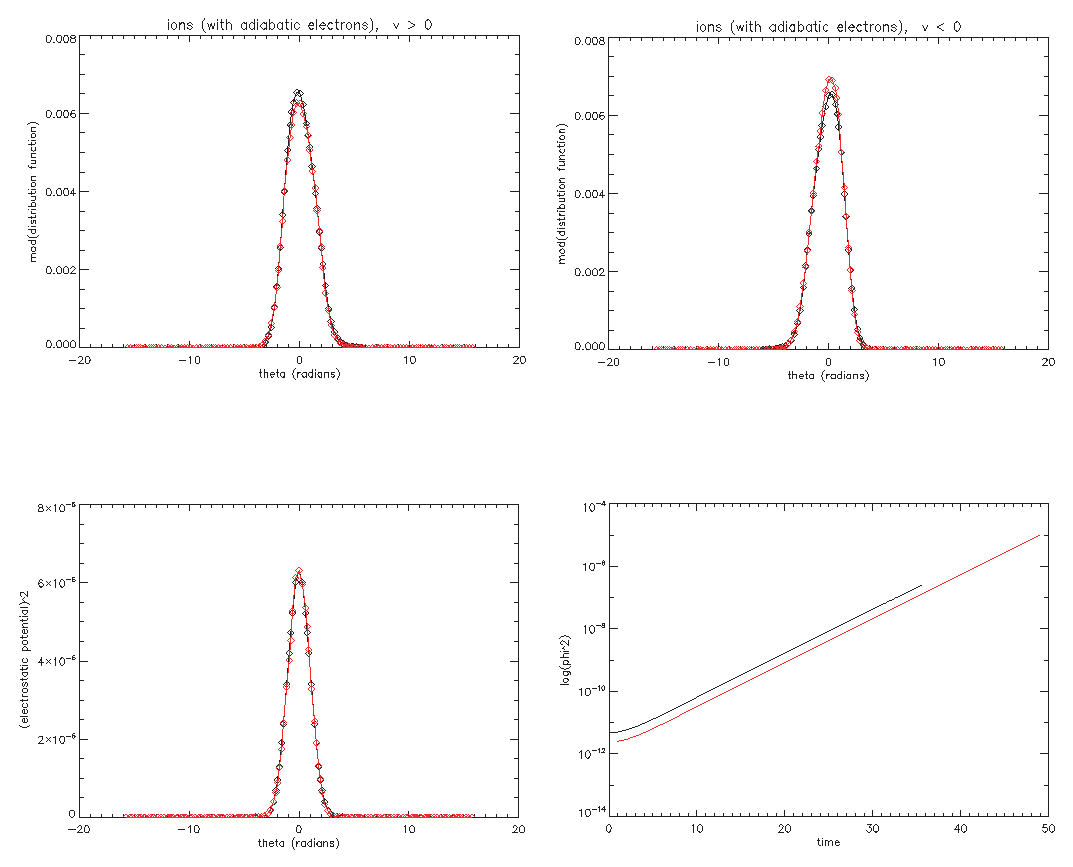
\epsfig{file=ae.eps,width=16cm,angle=0}
  \end{center}
  \caption{\textit{Plots demonstrating the results for adiabatic electron
      runs, when using a fixed time-step. The top row shows the distribution
      functions vs.\ poloidal angle $\theta$ for the ions with positive and
      negative parallel velocities, respectively. The plot at bottom-left is
      $|\phi|^2$ vs.\ $\theta$, and the bottom-right plot is $\phi^2$ vs.\
      time (with a logarithmic vertical scale). In all cases, the results
      using GS2's implicit algorithm are shown in black, while the
      corresponding results obtained using the new DG-RK algorithm are shown
      in red.}
    \label{fig:ae_results} }
\end{figure}

\begin{figure}[!p]
  \begin{center}
    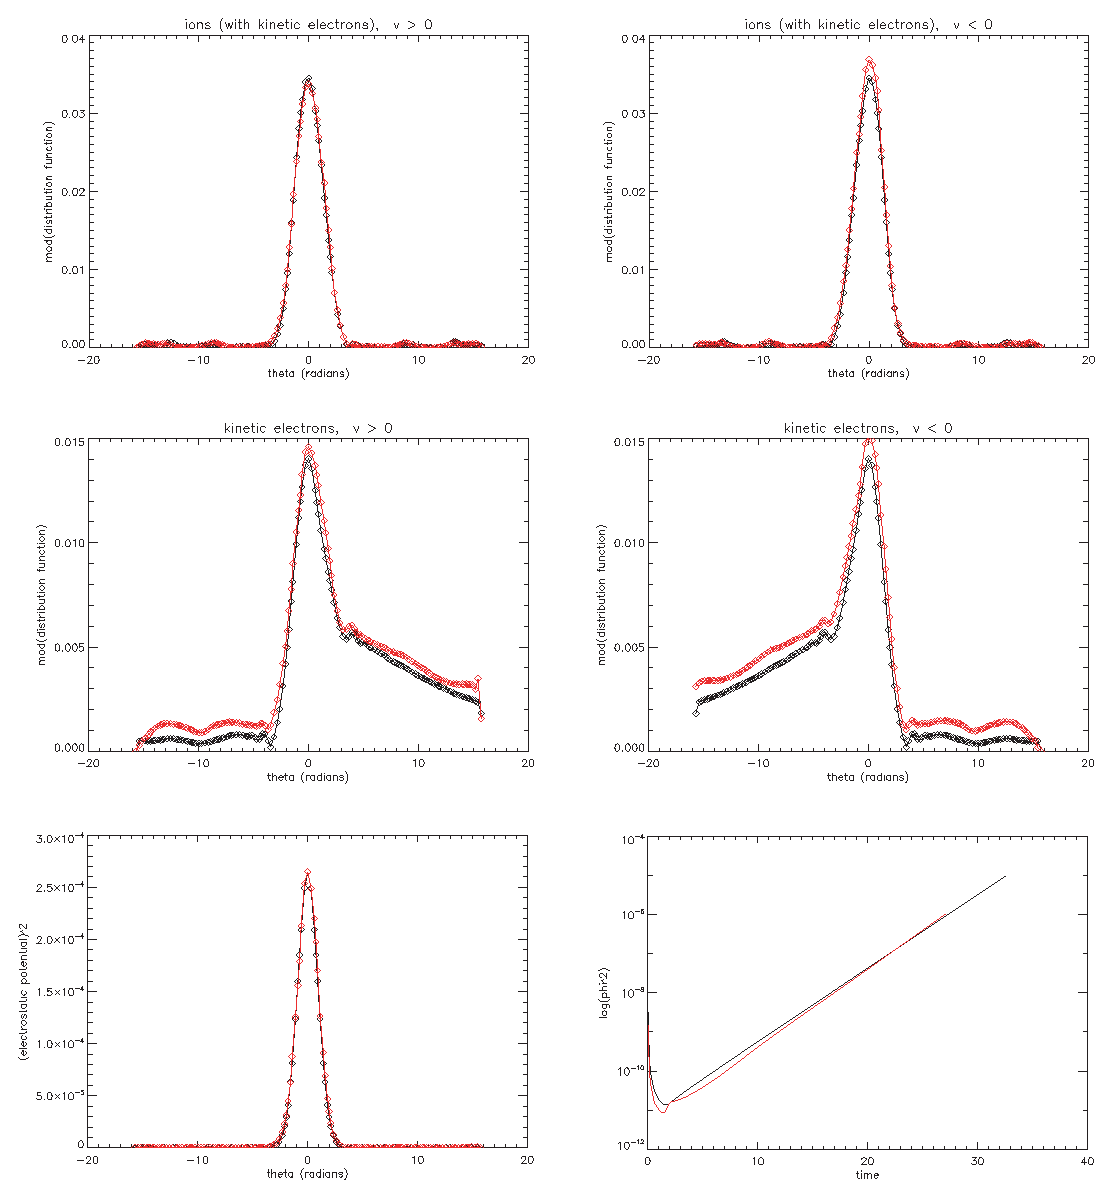
\epsfig{file=ke.eps,width=16cm,angle=0}
  \end{center}
  \caption{\textit{Plots demonstrating the results for kinetic electron runs,
      when using a fixed time-step. The top row shows the distribution
      functions vs.\ poloidal angle $\theta$ for the ions with positive and
      negative parallel velocities, respectively, while the middle row shows
      the corresponding electron distribution functions. The plot at
      bottom-left is $|\phi|^2$ vs.\ $\theta$, and the bottom-right plot is
      $\phi^2$ vs.\ time (with a logarithmic vertical scale). In all cases,
      the results using GS2's implicit algorithm are shown in black, while the
      corresponding results obtained using the new DG-RK algorithm are shown
      in red.}
    \label{fig:ke_results} }
\end{figure}

\subsection{Adaptive time-step results}

We noted mixed results when the algorithm described in
Section~\ref{sec:control} was invoked. The solution with adiabatic electrons
was excellent, with $\Delta t$ settling quickly down to 0.160, which is very
close to the value of $\Delta t_{\mbox{\scriptsize max}} = 0.162$ shown in
Table~\ref{tab:growthrates}. The growth rates also agreed with the previous
fixed time-step run. However, the kinetic electron case failed to converge;
Figure~\ref{fig:adaptivedt2} demonstrates the problem. The growth rate
calculation in GS2 depends on the present value of $\Delta t$, and so if this
jitters around, the growth rates also oscillate and the GS2 growth rate
convergence criterion is never met. Something in the physics of the problem
appears to cause the value of $R$ to oscillate around $f^3$ in small but
growing amplitude jumps, until $R$ becomes above 1.0, when the oscillations
reset back to small amplitude again, and this cycle repeats indefinitely.

The problem was alleviated by imposing a maximum allowed time-step that is
reduced automatically every time $R > 1$ is encountered, thus damping the
undesirable oscillations in $\Delta t$. The resulting $\Delta t = 0.00143$,
close to the previous $\Delta t_{\mbox{\scriptsize max}} = 0.00165$, and the
growth rates agree with the corresponding case in the Table.

\begin{figure}[!p]
  \begin{center}
    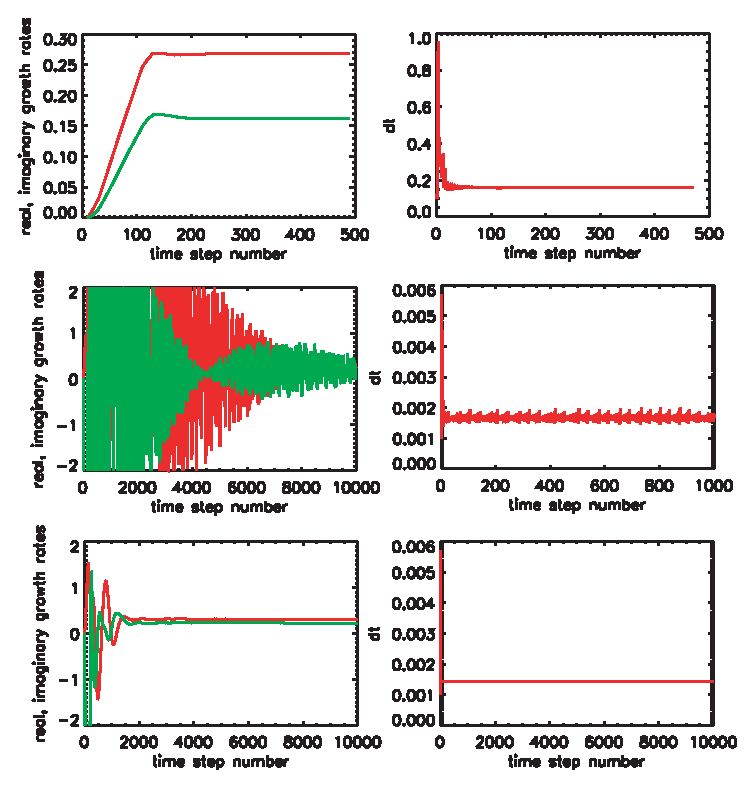
\epsfig{file=adaptivedt2.eps,height=16cm,angle=0}
  \end{center}
  \caption{\textit{Plots demonstrating the growth rate and time-step evolution for
    adiabatic (top) and kinetic (middle) electron cases, when using the adaptive
    time-step algorithm. The bottom plots show the kinetic electron case when
    the time-step is subject to additional damping as described in the text.}
  \label{fig:adaptivedt2} }
\end{figure}


\section{Concluding Remarks}

We have produced a version of GS2 with a working explicit scheme based on a
Discontinuous Galerkin finite element method combined with adaptive
Runge-Kutta time-advancement. The results presented above have demonstrated,
albeit for a reduced class of scenarios, that the new scheme reproduces the
results from the existing implicit scheme sufficiently closely to be a useful
addition to the code.

The DGGS2 Principal Investigator (Colin Roach) regards the project as having
been successful in its aim of implementing the DG scheme within GS2.
Notwithstanding the remaining work required to determine and correct the
causes of the problems with the trapped particle boundary conditions, this
project has resulted in a valuable complementary approach for GS2 users to
use.

In the future (outside of the HLST remit), the authors intend to complete the
trapped particle implementation, and to run additional tests to ensure that
the new scheme is useful in electromagnetic and non-linear scenarios. At that
point it will be possible to perform useful, large-scale tests of the
algorithm's capability, to see if the predicted savings in computational costs
are realised.

\section*{Acknowledgements}

This work was performed under the EFDA workprogramme 2009 under project
WP09-HPC-HLST and its continuations. The UK researchers' work was supported by
EPSRC grants EP/I501045 (as part of the RCUK Energy Programme), EP/H00212X/1
and EP/H002081/1, and the European Communities under the Contract of
Association between EURATOM and CCFE\@. The views and opinions expressed
herein do not necessarily reflect those of the European Commission. We would
like to thank the other members of the High Level Support Team for fruitful
discussions during the course of this and the preceding projects.

\begin{thebibliography}{99}

\bibitem{kotschenreuther}
M.~Kotschenreuther, G.~Rewoldt and W.~M.~Tang, Computer Physics
  Communications \textbf{88} (1995) 128

\bibitem{hammer}
Nicolay J.~Hammer and Roman Hatsky, \textit{Combining Runge-Kutta
  discontinuous Galerkin methods with various limiting methods}, IPP Report
IPP 5/124, Max-Planck Society (2010), \texttt{edoc.mpg.de/446381}

\bibitem{butcher}
John Butcher, \textit{Runga-Kutta methods}, Scholarpedia, 2(9):3147 (2007)

\bibitem{stoer_bulirsch}
J.~Stoer and R.~Bulirsch, \textit{$\S 7.2.5$, Introduction to Numerical Analysis, 3rd
  Edition.} Springer, 2002.

\bibitem{rkf45}
H.~A.~Watts and L.~F.~Shampine, Netlib library subroutine
\texttt{http://www.netlib.org/ode/rkf45.f}

%\bibitem{logbook23}
%P.~Knight, Logbook 23, pp.30-33

% \bibitem{manual}
% W.~Arter, \textit{GS2 Manual},
% /home/warter/gyrokinetics/docs/gs2/trunk/gs2\_manual.pdf. N.B.\
% This document remains unfinished, and the numbering therein is inconsistent and
% not unique. I have referred to page number \textit{n}\/ as either
% \textit{An}\/ or \textit{Bn}, depending on whether it is the first or second
% occurrence respectively of the given page number.

% \bibitem{dgreport}
% W.~Arter and P.~Knight, \textit{Implementing Discontinuous Galerkin Schemes in
%   GS2}, 
% /home/pknight/hpcff/hlst/gs2\_dg\_implementation20110331.pdf

\end{thebibliography}

\newpage
\appendix

\section{Gyrokinetic and Maxwell Field Equations in GS2}
%\author{C M Roach}
%\date{November 28, 2011}
%\maketitle

\subsection{\label{GKE} Gyrokinetic Equation and Perturbed Distribution
  Function}

In the absence of flows the linear electrostatic gyrokinetic equation is
derived for the perturbed distribution function for an isotropic equilibrium:
\[ f_{0s} = n_s(x) \left(\frac{m_s}{2\pi T_s(x)}\right)^{1.5} e^{-m_s
  v^2/2T_s(x)}
\]
where $n_s(x)$ and $T_s(x)$ represent the equilibrium temperature and density
on a given flux surface labelled by $x$. The perturbed distribution function
at next order in $\delta= \rho/L$ is given by:
\begin{equation}
f_{1s} = \frac{q_s \Phi_1}{m_s} \pd{f_{0s}}{E} +
g_s(\bfm{r},v_{\parallel},v_{\perp}) e^{-i\bfm{k.\rho_s}} \label{eq:f1}
\end{equation}
where the nonadiabatic part of the perturbed distribution function $g_s$ is
obtained from the linearised electromagnetic gyrokinetic equation:
\begin{align}
\frac{\partial g_s}{\partial t} + \left( v_{\parallel} \bfm{b} + \bfm{v_d}
\right). \grad{g_s} +C_s g_s & =  -q_s \pd{f_{0s}}{E} \pd{\chi}{t} +  \left\{
  \chi, f_{0s}\right\} \label{eq:gklin}
%+ \frac{\bfm{\grad_{\perp}} \chi \times \bfm{b}}{B} .\grad{f_{0s}} \\ 
\end{align}
where $\bfm{b}=\bfm{B_0}/B_0$, $Z_s=k_{\perp} \rho_s$, and:
\begin{align*}
\{ \chi,f_{0s} \} = \frac{1}{B} \grad_{\perp} \chi \times \bfm{b}
.\grad{f_{0s}} \hspace*{1cm}& \chi = \left( \Phi_1 - v_{\parallel}
  A_{\parallel} \right) J_0(Z) + \frac{m_s v_{\perp}^2}{q_s}
\frac{B_{\parallel}}{B} \frac{J_1(Z)}{Z} 
\end{align*}
$\Phi_1$ is perturbed electrostatic potential, $A_{\parallel}$ is perturbed
$\parallel$ magnetic potential, and $B_{\parallel}$ is perturbed $\parallel$
magnetic field.  $\bfm{v_d}$ contains equilibrium magnetic drifts:
\begin{align*}
 \bfm{v_d} = \frac{1}{\Omega_s} \bfm{b} \times
\left( \frac{\mu}{m} \grad{B} + v_{\parallel}^2 \bfm{b.}\grad{b} \right)
\end{align*}
The linear GKE in~(\ref{eq:gklin}) is equivalent to equation~(24) of
\cite{antonsen_PF1980}, which is the formulation of gyrokinetics that is
solved in GS2.  $g_s$ here corresponds to $h$ that is defined in
\cite{antonsen_PF1980}'s equation~(23), if we assume an isotropic equilibrium
distribution function that satisfies $\pd{f_{0s}}{\mu}=0$.

For numerical convenience, GS2 solves the gyrokinetic
equation~(\ref{eq:gklin}) for a modified form of the perturbed distribution
function, $h_s$:
\begin{align}
 h_s (\bfm{r}, E, \mu) & = g_s(\bfm{r}, E, \mu)  - \frac{q_s}{T_s} \Phi J_0(Z)
 f_{0s} - \frac{m_s v_{\perp}^2}{T_s} \frac{B_{\parallel}}{B} \frac{J_1(Z)}{Z}
 f_{0s} \label{eq:h}
\end{align}
Translation between $g_s$ and $h_s$ is conputed in the GS2 subroutine
g\_adjust.  Substituting (\ref{eq:h}) into (\ref{eq:gklin}) gives the
gyrokinetic equation in the form that is most closely related to how the GKE
is solved numerically in GS2:
\begin{align}
\frac{\partial h_s}{\partial t} + \left( v_{\parallel} \bfm{b} + \bfm{v_d}
\right). \grad{h_s} + C_s g_s & = q_s v_{\parallel} J_0(Z) \pd{f_{0s}}{E}
\pd{A_{\parallel}}{t}  \nonumber \\
& - f_{0s} \left( v_{\parallel} \bfm{b} + \bfm{v_d}
\right). \grad{ \left[ \frac{q_s}{T_s} \Phi J_0(Z) + \frac{m_s
      v_{\perp}^2}{T_s} \frac{B_{\parallel}}{B} \frac{J_1(Z)}{Z} \right]}
\nonumber \\
& + \left\{ \chi, f_{0s}\right\} 
\label{eq:gkl_gs2} 
%+ \frac{\bfm{\grad_{\perp}} \chi \times \bfm{b}}{B} .\grad{f_{0s}} \\ 
\end{align}
The terms on the LHS that involve $h_s$ are solved implicitly; the collision
term $C_s g_s$ is computed as a separate step using operator splitting; and
the source terms on the RHS correspond to the variable {\em source} that is
computed in subroutine set\_source in dist\_fn.f90.

Velocity space coordinates are $\mu=mv_{\perp}^2/(2B)$, $E=mv^2/2$ and
gyrophase angle $\gamma$. A volume element of velocity space $d^3v = v_{\perp}
dv_{\perp} dv_{\parallel} d \gamma$, and when the integrand is independent of
gyrophase this can be written in terms of two velocity coordinates as $d^3v =
2\pi v_{\perp} dv_{\perp} dv_{\parallel} = 2 \pi \frac{B d \mu dE}{\sqrt{2
    m_s(E-\mu B)}}$.

\subsection{\label{Maxwell} Maxwell's Field Equations in Gyrokinetics}

Perturbed electric and magnetic fields obtained from electrostatic and
magnetic potentials:
\begin{align}
\bfm{E_1} &= -\grad{\Phi} - \epsilon_0 \pd{A_{\parallel} \bfm{b}}{t} \\
\bfm{B_1} &= \bfm{\nabla} \times \left( A_{\parallel} \bfm{b} \right) + B_{\parallel} \bfm{b} 
\end{align}
$\Phi$ and $A_{\parallel}$ are determined self-consistently from Maxwell's
equations, neglecting the displacement current which is small in the
gyrokinetic orderings.

Poisson's equation reduces to the quasineutrality condition if we assume the
limit where $k_{\perp}^2 \lambda_D^2 \ll 1$.
\begin{align*}
& \sum_s \int d^3v \; q_s \left( q_s \Phi \pd{f_{0s}}{E} + g_s
  e^{-i\bfm{k.\rho_s}} \right)  = 0
\end{align*}
Gyrophase integration using $\frac{1}{ 2\pi} \int d\gamma e^{-i
  \bfm{k.\rho_s}} = J_0(Z_s)$ gives the GK Poisson equation:
\begin{align}
- \Phi \sum_s \frac{n_s q_s^2}{T_s}  +  \sum_s q_s \int d^3v J_0(Z_s) g_s  =
0 \label{eq:poisson}
\end{align}
Gyrokinetic orderings require that $B_{\parallel}$ satisfies perpendicular
force balance, as GK does not capture high frequency fast Alfv\`{e}n
waves. Some algebra gives the GK solution for the perpendicular component of
Amp\`{e}re's Law :
\begin{align}
\frac{B_{\parallel}}{B} & = -\frac{\mu_0}{B^2} \sum_s \int d^3v \; m_s
v_{\perp}^2 g_s \frac{J_1(Z_s)}{Z_s} & \label{eq:bpar}
\end{align}
More straightforwardly, the parallel component of Amp\`ere's law gives:
\begin{align}
k_{\perp}^2 A_{\parallel} & = \mu_0 \sum_s \int d^3v \; v_{\parallel} q_s g_s
J_0(Z_s) & \label{eq:apar}
\end{align}
It is clear that $B_1/B \propto \beta$, so that \textbf{$\bfm{\Rightarrow
    B_1}$ more important at high $\bfm{\beta}$}

\subsection{\label{GS2} Field Equations in Terms of $h_s$}

Substituting (\ref{eq:h}) for $g_s$ into (\ref{eq:poisson}-\ref{eq:apar}), and
using summation convention over species, $s$, gives
the field equations in terms of the distribution function $h_s$ that is evolved in GS2.\\
\small Quasineutrality to obtain $\Phi$:
\begin{align}
  & -\Phi \frac{n_s q_s^2}{T_s} + q_s \int d^3v J_0(Z_s) \left\{ h_s +
    \frac{q_s}{T_s} \Phi J_0(Z_s) f_{0s} + \frac{m_s v_{\perp}^2}{T_s}
    \frac{B_{\parallel}}{B} \frac{J_1(Z_s)}{Z_s} f_{0s} \right\} = 0 \nonumber
  \\
  & \Phi \left( \frac{n_s q_s^2}{T_s} - \frac{q_s^2}{T_s} \int d^3v J_0^2(Z_s)
    f_{0s} \right) = q_s \int d^3v J_0(Z_s) h_s + \frac{B_{\parallel}}{B}
  \frac{q_s m_s}{T_s} \int d^3v v_{\perp}^2 \frac{J_0(Z_s) J_1(Z_s)}{Z_s}
  f_{0s} \label{eq:poissh}
\end{align}
Perpendicular force balance determines $B_{\parallel}$:
\begin{align}
  & \frac{B_{\parallel}}{B} = -\frac{\mu_0}{B^2} \int d^3v \; m_s v_{\perp}^2
  \frac{J_1(Z_s)}{Z_s} \left\{ h_s + \frac{q_s}{T_s} \Phi J_0(Z_s) f_{0s} +
    \frac{m_s v_{\perp}^2}{T_s} \frac{B_{\parallel}}{B} \frac{J_1(Z_s)}{Z_s}
    f_{0s} \right\} \nonumber \\
  & \frac{B_{\parallel}}{B} \left( 1 + \frac{\mu_0}{B^2} \frac{m_s^2 }{T_s}
    \int d^3v \; v_{\perp}^4 \frac{J_1^2(Z_s)}{Z_s^2} f_{0s}\right) =
  -\frac{\mu_0 m_s}{B^2} \int d^3v \; v_{\perp}^2 \frac{J_1(Z_s)}{Z_s} h_s -
  \frac{\mu_0 m_s q_s}{B^2 T_s} \Phi \int d^3v \; v_{\perp}^2 \frac{J_0(Z_s)
    J_1(Z_s)}{Z_s} f_{0s} \label{eq:bparh}
\end{align} 
The parallel component of Amp\`ere's law gives $A_{\parallel}$:
\begin{align}
  & k_{\perp}^2 A_{\parallel} = \mu_0 q_s \int d^3v \; v_{\parallel} J_0(Z_s)
  \left\{ h_s + \frac{q_s}{T_s} \Phi J_0(Z_s) f_{0s} + \frac{m_s
      v_{\perp}^2}{T_s} \frac{B_{\parallel}}{B} \frac{J_1(Z_s)}{Z_s}
    f_{0s} \right\} \nonumber \\
  & k_{\perp}^2 A_{\parallel} = \mu_0 q_s \int d^3v \; v_{\parallel} J_0(Z_s)
  h_s \hspace*{1cm} {\rm \; (integrals\; odd \; in \;} v_{\parallel} \; {\rm
    vanish )} \label{eq:aparh}
\end{align}
\normalsize The above three field equations~(\ref{eq:poissh}-\ref{eq:aparh})
are used to obtain $\Phi$, $B_{\parallel}$ and $A_{\parallel}$ in GS2.
Clearly equations (\ref{eq:poissh}) and \ref{eq:bparh}) are coupled.

\subsubsection{Adiabatic Species Approximations}

In the adiabatic approximation, the perturbed distribution function for
species $a$ is given by:
\begin{equation} 
f_{1a} = \frac{q_a \left(\Phi_1 - {\cal F}_m \right) f_{0a}}{T_a} 
\end{equation}
where ${\cal F}_m$ is a model velocity independent spatial surface average
that depends on the nature of the perturbation.

\begin{table}[h]
\begin{center}
 \begin{tabular}{|ccl|}
\hline
Physics Model & ${\cal F}_{m}$ at $k_y=0$ & adiabatic\_option \\
\hline
& & \\
ion response to short wavelength ETG &  0 & `iphi00=0' \\ & & \\
electron response to long wavelength ITG & ${\cal F}_{m} = \flav{\Phi_1}$ & `iphi00=2' \\
%`dimits`   &  $\frac{\oint \frac{\rho_k}{a_k +a_a} d\theta }{\oint  \frac{a_k}{(a_k + a_a)} d\theta}$ & 'experimental' \\ \\
%`flavcmr`  &  $\frac{\oint \frac{\rho_k}{a_k +a_a} dl}{\oint  \frac{a_k}{(a_k + a_a)} dl}$ & CMR's minor modification to 'iphi00=2` \\
%& & replacing $dl dA =J d\theta$ with $dl = d\theta / (\gradpar \theta)$ \\
\hline
\end{tabular}
\end{center}
\caption{\label{tab:adgs2} Physical adiabatic model options for ${\cal F}_m$,
  which is chosen in GS2 using the variable adiabatic\_option. In all models
  ${\cal F}_m = 0$ for any finite $k_y$. $\flav{.}$ denotes the flux-surface
  average operator.}
\end{table}

For Maxwellian equilibrium, $f_{1a}$ is independent of gyrophase and the sign
of $v_{\parallel}$: $f_{1a}$, therefore, contributes to the perturbed charge
density, but not to the perturbed current density.  Including adiabatic
species modifies the field equations, and the quasineutrality
condition~(\ref{eq:poissh}) is modified as follows, to give: \small
\begin{align}
  \Phi \left( \frac{n_s q_s^2}{T_s} + \frac{n_a q_a^2}{T_a} -
    \frac{q_s^2}{T_s} \int d^3v J_0^2(Z_s) f_{0s} \right) - \frac{n_a
    q_a^2}{T_a} {\cal F}_m = q_s \int d^3v J_0(Z_s) h_s +
  \frac{B_{\parallel}}{B} \frac{q_s m_s}{T_s} \int d^3v v_{\perp}^2
  \frac{J_0(Z_s) J_1(Z_s)}{Z_s} f_{0s} \label{eq:poissha}
\end{align}
\normalsize When adiabatic species are included in the equations for
quasineutrality~(\ref{eq:poissha}), perpendicular force
balance~(\ref{eq:bparh}) and Amp\`ere's law (\ref{eq:aparh}), the implicit
species sums over $s$ exclude adiabatic species and are \textbf{only} over
fully kinetic species.

In the adiabatic model where ${\cal F}_{m} = \flav{\Phi_1}$, we obtain the
finite value of $\flav{\Phi_1}$ (for $k_y=0$) from
equation~(\ref{eq:poissha}), as follows: \small
\begin{align}
  \Phi & = \frac{q_s \int d^3v J_0(Z_s) h_s + \frac{B_{\parallel}}{B}
    \frac{q_s m_s}{T_s} \int d^3v v_{\perp}^2 \frac{J_0(Z_s) J_1(Z_s)}{Z_s}
    f_{0s} + \frac{n_a q_a^2}{T_a} \flav{\Phi}} {\left( \frac{n_s q_s^2}{T_s}
      + \frac{n_a q_a^2}{T_a} - \frac{q_s^2}{T_s}
      \int d^3v J_0^2(Z_s) f_{0s} \right)} \nonumber \\
  \flav{\Phi} & = \frac{\flav{ \frac{q_s \int d^3v J_0(Z_s) h_s +
        \frac{B_{\parallel}}{B} \frac{q_s m_s}{T_s} \int d^3v v_{\perp}^2
        \frac{J_0(Z_s) J_1(Z_s)}{Z_s} f_{0s} } {\left( \frac{n_s q_s^2}{T_s} +
          \frac{n_a q_a^2}{T_a} - \frac{q_s^2}{T_s} \int d^3v J_0^2(Z_s)
          f_{0s} \right)}}} {1-\flav{ \frac{ \frac{n_a q_a^2}{T_a}}{\left(
          \frac{n_s q_s^2}{T_s} + \frac{n_a q_a^2}{T_a} - \frac{q_s^2}{T_s}
          \int d^3v J_0^2(Z_s)
          f_{0s} \right)}}} \nonumber \\
  \Rightarrow {\cal F}_m & = \flav{\Phi} = \frac{\flav{ \frac{q_s \int d^3v
        J_0(Z_s) h_s + \frac{B_{\parallel}}{B} \frac{q_s m_s}{T_s} \int d^3v
        v_{\perp}^2 \frac{J_0(Z_s) J_1(Z_s)}{Z_s} f_{0s} } {\left( \frac{n_s
            q_s^2}{T_s} + \frac{n_a q_a^2}{T_a} - \frac{q_s^2}{T_s} \int d^3v
          J_0^2(Z_s) f_{0s} \right)}}} {\flav{ \frac{\frac{n_s q_s^2}{T_s} -
        \frac{q_s^2}{T_s} \int d^3v J_0^2(Z_s) f_{0s} }{\left( \frac{n_s
            q_s^2}{T_s} + \frac{n_a q_a^2}{T_a} - \frac{q_s^2}{T_s} \int d^3v
          J_0^2(Z_s) f_{0s} \right)}}} \label{eq:phiavg}
\end{align}
\normalsize

\subsection{Implementation of Field Equations in GS2}

\subsubsection{GS2 Normalisations}

All GS2 variables are normalised according to standard normalisations given in
Table~\ref{tab:norm}.

\small
\linespread{1.5}
\begin{table}[htb]
\begin{tabular}{|l|l|l|}
\hline
Quantity & Normalised Physical Quantities in GS2 &  Comments \\
\hline
Normalisation Quantities$^{\ast}$ & $n_{\rm ref}$, $T_{\rm ref}$, $m_{\rm
  ref}$, $q_{\rm ref}$ & reference $n$, $T$, $m$ and charge $q$ \\
                                  & $B_{\rm ref}$, $L_{\rm ref}$ & reference
                                  equ'm $B$ and length $L$ \\
Thermal Velocity$^{1}$ & $v_t = \sqrt{\frac{2 T_{\rm ref}}{m_{\rm ref}}}$  & \\
Species Thermal Velocity & $v_{ts}=\sqrt{\frac{\g{T_s}}{\g{m_s}}} v_t$ & \\
Equilibrium Dist Fn & $f_{0s}=n_s f_{0}$, Maxwellian $f_0$, $\int d^3v f_0 = 1$ &   \\
\hline
Equilibrium Quantities & $\g{n_s}=\frac{n_s}{n_{\rm ref}}$, $\g{T_s} =
\frac{T_s}{T_{\rm ref}}$, $\g{m_s} = \frac{m_s}{m_{\rm ref}}$ & \\
Equilibrium $B$ & $\g{B}=\frac{B}{\n{B}}$ & \\
Equilibrium Gradients & $\gradeq=\n{L} \grad$ & \\
Velocity Variable        & $\g{v} = \frac{v}{v_{ts}}$  & velocity variable for
species $s$ \\
Energy & $\g{E} = \frac{v^2}{v_{ts}^2} = \g{v}^2$ & \\
Pitch Angle & $\g{\lambda} = \frac{\g{v_{\perp}}^2}{\g{B} \g{v}^2}$ & $\lambda
= \frac{\mu}{E}$ \\
Larmor Radius Quantities & $\n{\rho} = \frac{\n{m} v_t}{\n{q} \n{B}}$ &
normalises $\perp$ lengths \\
Beta &  $\g{\beta} = \frac{2 \mu_0 \n{n} \n{T}}{\n{B}^2}$ & in GS2 field equations \\
Time &  $\g{t} = \frac{t v_t}{\n{L}}$ & \\
Frequency &  $\g{\omega} = \frac{ \omega \n{L}}{v_t}$ & \\
Parallel Gradients & $\ggp = \nabla_{\parallel} \n{L}$ &  \\
Perpendicular Gradients & $\gperp = \n{\rho}\grad_{\perp}$, or  $\g{k_{\perp}}
= k_{\perp} \n{\rho}$ &  \\
$k_y$ & $\g{k_y} = \frac{n_0 \n{\rho}}{\n{L}} \dd{\rho_n}{\psi_n}$ & $n_0$ is
toroidal mode number, \\
& & $\rho_n$ is radial flux label for equ'm derivatives \\
& & $\psi_n = \frac{\psi}{\n{B} \n{L}^2}$ is normalised poloidal flux\\ 
Perturbed $\Phi$ & $\g{\Phi} = \frac{\n{q} \Phi}{\n{T}} \frac{\n{L}}{\n{\rho}}$ & \\
Adiabatic ${\cal F}_m$  & $\g{F_m} = 
\begin{array}{|ll}
\frac{\n{q} \flav{\Phi}}{\n{T}} \frac{\n{L}}{\n{\rho}}, \;{\rm or}\; 0  & {\rm
  for}\; k_y=0 \\
0 & {\rm for}\; k_y \ne 0\\ \end{array}$ & NB ${\cal F}_m$ is depends on adiabatic model\\
Perturbed $B_{\parallel}$ & $\g{B_{\parallel}} =
\frac{B_{\parallel}}{B}\frac{\n{L}}{\n{\rho}}  \ne
\frac{B_{\parallel}}{\n{B}}\frac{\n{L}}{\n{\rho}}$&  \\
%Perturbed $A_{\parallel}$ & $\g{A_{\parallel}} =
%\frac{A_{\parallel}\n{L}}{\n{\rho}^2 \n{B}}$ &  follows from $\g{B_{\perp}} =
%\frac{B_{\perp} \n{L}}{\n{B} \n{\rho}}$  \\
Perturbed $A_{\parallel}$ & $\g{A_{\parallel}} = \frac{\n{q} v_t
  A_{\parallel}}{\n{T}} \frac{\n{L}}{\n{\rho}} = \frac{2
  A_{\parallel}}{\n{\rho} \n{B}} \frac{\n{L}}{\n{\rho}}$ &  follows from $\g{v
  A_{\parallel}} = \sqrt{\frac{T_s}{m_s}} \frac{v}{v_{ts}} \frac{\n{q} v_t
  A_{\parallel}}{\n{T}} \frac{\n{L}}{\n{\rho}}$  \\
Perturbed Dist Fn & $\g{h_s} = \frac{h_s}{f_{0s}} \frac{L_{\rm ref}}{\rho_{\rm
    ref}} = \frac{h_s}{\g{n_s}\n{n} f_{0}} \frac{L_{\rm ref}}{\rho_{\rm ref}}$
& $\g{h_s}$ stored in GS2 variable g\\
\hline
\end{tabular}
\caption{\label{tab:norm} All GS2 variables are normalised dimensionless
  quantities, and the general normalisation rules are given in the table. 
  $^{\ast}$ The dimensional normalisation parameters do not appear in the code. 
  $^1$ Internally GS2 always uses $v_t = \sqrt{2T_{\rm ref}/m_{\rm ref}}$, but
  there is a (potentially confusing) option to allow output times
  and frequencies to be normalised using  $v_t = \sqrt{T_{\rm ref}/m_{\rm ref}}$.}
\end{table}
We now use Table~\ref{tab:norm} to normalise the magnetic drifts:
\begin{align*}
  \bfm{v_d} & = \frac{1}{\Omega_s} \bfm{b} \times \left( \frac{\mu}{m}
    \grad{B} + v_{\parallel}^2 \bfm{b.}\grad \bfm{b} \right) =
  \frac{v_{ts}^2}{\n{L} \Omega_s} \bfm{b} \times \left(
    \frac{\g{v_{\perp}^2}}{2B} \gradeq{B} + \g{v_{\parallel}}^2
    \bfm{b.}\gradeq \bfm{b} \right) \\
  \bfm{v_d} & = \frac{\g{T_s}\n{\rho} v_t}{\g{q_s}\n{L}} \bfm{b} \times \left(
    \frac{\g{v_{\perp}^2}}{2B} \gradeq{B} + \g{v_{\parallel}}^2
    \bfm{b.}\gradeq \bfm{b} \right)
\end{align*}
to obtain:
\begin{align}
  \bfm{v_d}.\grad_{\perp} & = \frac{\g{T_s} v_t}{\g{q_s}\n{L}} \bfm{b} \times
  \left( \frac{\g{v_{\perp}^2}}{2B} \gradeq{B} + \g{v_{\parallel}}^2
    \bfm{b.}\gradeq \bfm{b} \right).\gperp
\label{eq:vdnorm}
\end{align}
and the gyrokinetic electromagnetic potential:
\begin{align}
  \chi & = \left( \Phi_1 - v_{\parallel} A_{\parallel} \right) J_0(Z) +
  \frac{m_s v_{\perp}^2}{q_s} \frac{B_{\parallel}}{B} \frac{J_1(Z)}{Z}
  \nonumber \\
  \chi & = \frac{\n{\rho}}{\n{L}} \frac{\n{T}}{\n{q}} \left( \g{\Phi} J_0(Z) -
    \sqrt{\frac{\g{T_s}}{\g{m_s}}} \g{v_{\parallel}} \g{A_{\parallel}} J_0(Z)
    + \frac{2 \g{T_s}}{\g{q_s}} \g{v_{\perp}^2} \g{B_{\parallel}}
    \frac{J_1(Z)}{Z} \right) \label{eq:chinorm}.
\end{align}

\linespread{1}
\normalsize
\subsubsection{Normalised Field Equations}

We now multiply all the field equations
(\ref{eq:poissha},\ref{eq:bparh},\ref{eq:aparh}) by $\n{L}/\n{\rho}$ to remove
the small ordering factor that scales these equations, and reexpress the
equations in terms of the GS2 normalisations.

\subsubsection*{Quasineutrality}
The quasineutrality equation~(\ref{eq:poissha}) can be expressed:
 \begin{align*}
   LHS & = \n{n} \n{q} \left[ \g{\Phi} \frac{\g{n_s} \g{q_s}^2}{\g{T_s}}
     \left( 1 - \int d^3v \; f_0 \; J_0^2(Z_s) \right) + \frac{\g{n_a}
       \g{q_a}^2}{\g{T_a}} \left( \g{\Phi} - \g{F_m} \right) \right] \\
   RHS &= \n{n} \n{q} \g{n_s} \g{q_s} \left[ \int d^3v \;f_0 \; J_0(Z_s)
     \frac{\n{L}}{\n{\rho}} \frac{h_s}{f_{0s}} + \frac{B_{\parallel}}{B}
     \frac{\n{L}}{\n{\rho}} \int d^3v \;f_{0} \;2\frac{v_{\perp}^2}{v_{ts}^2}
     \frac{J_0(Z_s) J_1(Z_s)}{Z_s} \right]
\end{align*}
to give:
\begin{align}
  \g{\Phi} \frac{\g{n_s} \g{q_s}^2}{\g{T_s}} \int d^3v \; f_0 \; \left( 1
    -J_0^2(Z_s) \right) + \frac{\g{n_a} \g{q_a}^2}{\g{T_a}} \left( \g{\Phi} -
    \g{F_m} \right) & = \; \g{n_s} \g{q_s} \int d^3v \;f_0 \; J_0(Z_s) \g{h_s}
  + \g{B_{\parallel}} \g{n_s} \g{q_s} \int d^3v \;f_{0} \; \frac{ 2
    \g{v_{\perp}}^2 J_0(Z_s) J_1(Z_s)}{Z_s} \label{eq:npoiss}.
\end{align}
The $\Phi$ average term of equation~(\ref{eq:phiavg}) used in one adiabatic
response model is expressed in normalised variables as:
\begin{align}
  \flav{\g{\Phi}} & = \frac{\flav{ \frac{\g{q_s} \g{n_s} \int d^3v f_0
        J_0(Z_s) \g{h_s} + \g{B_{\parallel}} \g{q_s} \g{n_s} \int d^3v f_{0}
        \frac{2 \g{v_{\perp}}^2 J_0(Z_s) J_1(Z_s)}{Z_s} } {\left(
          \frac{\g{n_s} \g{q_s}^2}{\g{T_s}} \left( 1 - \int d^3v f_{0}
            J_0^2(Z_s) \right) + \frac{\g{n_a} \g{q_a}^2}{\g{T_a}} \right)}}}
  {\flav{ \frac{ \frac{\g{n_s} \g{q_s}^2}{\g{T_s}} \left( 1 - \int d^3v f_{0}
          J_0^2(Z_s) \right) } {\left( \frac{\g{n_s} \g{q_s}^2}{\g{T_s}}
          \left( 1 - \int d^3v f_{0} J_0^2(Z_s) \right) + \frac{\g{n_a}
            \g{q_a}^2}{\g{T_a}} \right)}}} \label{eq:nphiavg}
\end{align}

\subsubsection*{Perpendicular Force Balance}
Following the same procedure for perpendicular force balance,
equation~(\ref{eq:bparh}), gives:
\begin{align*}
  LHS & = \g{B_{\parallel}} \left( 1 + \frac{\mu_0 \n{n} \g{n_s}}{\n{B}^2
      \g{B}^2} \frac{m_s^2 v_{ts}^4}{T_s} \int d^3v \; f_{0} \;
    \frac{v_{\perp}^4}{v_{ts}^4} \frac{J_1^2(Z_s)}{Z_s^2} \right) =
  \g{B_{\parallel}} \left( 1 + \left( \frac{2 \mu_0 \n{n} \n{T}}{\n{B}^2}
    \right) \frac{\g{n_s} \g{T_s}}{\g{B}^2}
    \int d^3v \;  f_{0}  \frac{2 \g{v_{\perp}}^4 J_1^2(Z_s)}{Z_s^2} \right) \\
  & = \g{B_{\parallel}} \left( 1 + \g{\beta} \frac{\g{n_s} \g{T_s}}{\g{B}^2}
    \int d^3v \;  f_{0} \frac{2 \g{v_{\perp}}^4 J_1^2(Z_s)}{Z_s^2} \right) \\
  RHS & = -\frac{\mu_0 n_s m_s v_{ts}^2}{\n{B}^2 \g{B}^2} \int d^3v \; f_0
  \frac{v_{\perp}^2}{v_{ts}^2} \frac{J_1(Z_s)}{Z_s} \g{h_s} - \frac{\mu_0 m_s
    n_s v_{ts}^2}{B^2} \frac{\g{q_s}}{\g{T_s}}
  \left(\frac{\n{q}\Phi}{\n{T}}\right) \int d^3v \; f_{0}
  \frac{v_{\perp}^2}{v_{ts}^2} \frac{J_0(Z_s) J_1(Z_s)}{Z_s} \\
  & = - \g{\beta} \left( \frac{\g{n_s} \g{T_s}}{\g{B}^2} \int d^3v \; f_0
    \frac{\g{v_{\perp}^2} J_1(Z_s)}{Z_s} \g{h_s} + \g{\Phi} \frac{\g{n_s}
      \g{q_s}}{\g{B}^2} \int d^3v \; f_{0} \frac{\g{v_{\perp}^2} J_0(Z_s)
      J_1(Z_s)}{Z_s} \right)
\end{align*}
and GS2's dimensionless perpendicular force balance equation is:
\begin{align}
  \g{B_{\parallel}} \left( 1 + \g{\beta} \frac{\g{n_s} \g{T_s}}{\g{B}^2} \int
    d^3v \; f_{0} \;2 \frac{\g{v_{\perp}^4} J_1^2(Z_s)}{Z_s^2} \right) & = -
  \g{\beta} \frac{\g{n_s} \g{T_s}}{\g{B}^2} \int d^3v \; f_0
  \frac{\g{v_{\perp}^2} J_1(Z_s)}{Z_s} \g{h_s} - \g{\Phi} \frac{\g{\beta}}{2}
  \frac{\g{n_s} \g{q_s}}{\g{B}^2} \int d^3v \; f_{0} \frac{2 \g{v_{\perp}^2}
    J_0(Z_s) J_1(Z_s)}{Z_s}
\label{eq:nperpf}
\end{align}

\subsubsection*{Parallel Amp\`ere's Law}
In terms of normalised quantities the parallel Amp\`ere's law,
equation~(\ref{eq:aparh}) we have:
\begin{align*}
  LHS & = \frac{\n{B}}{2 \n{\rho}} \left( k_{\perp} \n{\rho} \right)^2 \left(
    \frac{2A_{\parallel}}{\n{B} \n{\rho}} \right) \frac{\n{L}}{\n{\rho}} =
  \frac{\n{B}}{2\n{\rho}} \g{k_{\perp}}^2 \g{A_{\parallel}} = \frac{\n{q}
    \n{B}^2}{2 \n{m} v_t} \g{k_{\perp}}^2 \g{A_{\parallel}} \nonumber \\
  RHS & = \mu_0 \n{n} \n{q} v_{t} \g{n_s} \g{q_s}
  \sqrt{\frac{\g{T_s}}{\g{m_s}}} \int d^3v \; f_0 \frac{v_{\parallel}}{v_{ts}}
  J_0(Z_s) \left( \frac{h_s \n{L}}{f_{0s} \n{\rho}} \right).
\end{align*}
The normalised parallel Amp\`ere Law is:
\begin{align}
  \g{k_{\perp}}^2 \g{A_{\parallel}} & = \frac{4 \mu_0 \n{n} \n{T}}{\n{B}^2}
  \g{n_s} \g{q_s} \sqrt{\frac{\g{T_s}}{\g{m_s}}} \int d^3v \; f_0
  \g{v_{\parallel}} J_0(Z_s)
  \g{h_s} \nonumber \\
  \g{k_{\perp}}^2 \g{A_{\parallel}} & = 2 \g{\beta} \g{n_s} \g{q_s}
  \sqrt{\frac{\g{T_s}}{\g{m_s}}} \int d^3v \; f_0 \g{v_{\parallel}} J_0(Z_s)
  \g{h_s} \label{eq:napar}
\end{align}

$\g{\Phi}$ and $\g{B_{\parallel}}$ can be determined from equations
(\ref{eq:npoiss}) and (\ref{eq:nperpf}), explicitly in terms of the perturbed
distribution functions. Substituting for the species summed velocity integrals
makes the algebra more compact, and here we will use the appropriate GS2
variables.

\subsubsection{Species Summed Velocity Integrals in GS2}
Various species summed velocity space integrals appear in
equations~(\ref{eq:npoiss}-\ref{eq:napar}), and the GS2 variables that contain
them are given in Table~\ref{tab:gs2_vints}.

\small
\linespread{2}
\begin{table}[htb]
\begin{center}
\begin{tabular}{|l|l|}
  \hline
  Species Summed Velocity Integrals & Variable Name\\
  \hline
  $\frac{\g{n_s} \g{q_s}^2}{\g{T_s}} \int d^3v \; f_0 \; \left( 1 - J_0^2(Z_s)
  \right) + \frac{\g{n_a} \g{q_a}^2}{\g{T_a}} $ & GAMTOT \\  
  $\g{n_s} \g{q_s}  \int d^3v  \;f_{0}  \frac{2 \g{v_{\perp}}^2 J_0(Z_s)
    J_1(Z_s)}{Z_s}$ & GAMTOT1 \\ 
  $\g{n_s} \g{T_s} \int d^3v \;  f_{0} \frac{2 \g{v_{\perp}}^4
    J_1^2(Z_s)}{Z_s^2}$ & GAMTOT2 \\ 
  $\frac{{\rm GAMTOT} {- \frac{\g{n_a} \g{q_a}^2}{\g{T_a}}}}
    {{\rm GAMTOT}}$ & GAMTOT3 \\ 
    $\g{n_s} \g{q_s} \int d^3v \;f_0 \; J_0(Z_s)  \g{h_s}$ & ANTOT \\
    $2 \g{\beta} \g{n_s} \g{q_s} \sqrt{\frac{\g{T_s}}{\g{m_s}}} \int d^3v \;
    f_0 \; \g{v_{\parallel}} J_0(Z_s) \g{h_s}$ & ANTOTA \\ 
    $\g{n_s} \g{T_s} \int d^3v \; f_0  \frac{\g{v_{\perp}}^2 J_1(Z_s)}{Z_s}
    \g{h_s}$ & ANTOTP \\
    \hline
\end{tabular}
\caption{\label{tab:gs2_vints} These velocity space integrals are calculated
  in GS2 routines in dist\_fn.f90.  GAMTOT, GAMTOT1, GAMTOT2 (and GAMTOT3 if
  there are adiabatic species) are computed at initialisation in routine
  init\_fieldeq. ANTOT, ANTOTA, and ANTOTP involve integrals over the evolving
  perturbed distribution function, and are computed in routine getan. Note
  that the GS2 variable ${\rm AJ1} = J_1(Z_s)/Z_s$.}
\end{center}
\end{table}
\linespread{1}

\subsubsection{GS2 Field Equations}
Equations (\ref{eq:npoiss}), (\ref{eq:nperpf}) and (\ref{eq:napar}) gives
$\g{\Phi}$, $\g{B_{\parallel}}$ and $\g{A_{\parallel}}$ explicitly in terms of
the perturbed distribution functions.
\begin{align} 
  \g{\Phi} & = \frac{\left( 1 + \frac{\g{\beta}}{\g{B}^2} {\rm GAMTOT2}
    \right) \left( {\rm ANTOT} + \frac{\g{n_a} \g{q_a}^2 \g{F_m}}{\g{T_a}}
    \right) - \frac{\g{\beta}}{\g{B}^2} {\rm ANTOTP}.{\rm GAMTOT1}} {\left( 1
      + \frac{\g{\beta}}{\g{B}^2} {\rm GAMTOT2} \right).{\rm GAMTOT} +
    \frac{\g{\beta}}{2\g{B}^2} {\rm GAMTOT1}^2} \label{eq:phigs2}\\
  \g{B_{\parallel}} & = -\g{\beta} \frac{\left( {\rm GAMTOT}.{\rm ANTOTP} +
      {\rm GAMTOT1}.\left( {\rm ANTOT} + \frac{\g{n_a} \g{q_a}^2
          \g{F_m}}{\g{T_a}} \right)/2 \right) } {\left( \g{B}^2 + \g{\beta}
      {\rm GAMTOT2} \right) .{\rm GAMTOT} +
    \g{\beta} {\rm GAMTOT1}^2/2} \label{eq:bpargs2}\\
  \g{A_{\parallel}} & = \frac{{\rm
      ANTOTA}}{\g{k_{\perp}}^2} \label{eq:apargs2}
\end{align}

The $\g{F_m}= \flav{\Phi}$ term used in one adiabatic model, can be expressed
in terms of GS2 variables using~(\ref{eq:nphiavg}):
\begin{align}
  \flav{\g{\Phi}} & = \frac{\flav{ \frac{ {\rm ANTOT} + \g{B_{\parallel}}.{\rm
          GAMTOT1} } {{\rm GAMTOT} }}} {\flav{ \frac{ {\rm GAMTOT
          -\frac{\g{n_a} \g{q_a}^2}{\g{T_a}} }}{{\rm
          GAMTOT}}}} \label{eq:phiavggs2_0}.
\end{align}
A more convenient but cumbersome expression, independent of
$\g{B_{\parallel}}$, can be obtained from equation~(\ref{eq:phigs2}):
\begin{align}
  \flav{\g{\Phi}} & = \frac{\flav{\frac{\left( 1 + \frac{\g{\beta}}{\g{B}^2}
          {\rm GAMTOT2} \right) {\rm ANTOT} - \frac{\g{\beta}}{\g{B}^2} {\rm
          ANTOTP}.{\rm GAMTOT1}} {\left( 1 + \frac{\g{\beta}}{\g{B}^2} {\rm
            GAMTOT2} \right).{\rm GAMTOT} + \frac{\g{\beta}}{2\g{B}^2} {\rm
          GAMTOT1}^2}}} {\flav{1 - \frac{\g{n_a} \g{q_a}^2}{\g{T_a}}
      \flav{\frac{\left( 1 + \frac{\g{\beta}}{\g{B}^2} {\rm GAMTOT2} \right)}
        {\left( 1 + \frac{\g{\beta}}{\g{B}^2} {\rm GAMTOT2} \right).{\rm
            GAMTOT} + \frac{\g{\beta}}{2\g{B}^2} {\rm GAMTOT1}^2}} }}
\label{eq:phiavggs2}
\end{align}
In the $\g{\beta}=0$ limit $\g{B_{\parallel}}$ must vanish, and
(\ref{eq:phiavggs2_0}) and (\ref{eq:phiavggs2}) both simplify to give:
\begin{align}
  \flav{\g{\Phi}} & = \frac{\flav{ \frac{ {\rm ANTOT}}{{\rm GAMTOT}}}} {\flav{
      \frac{\left( {\rm GAMTOT} - \frac{\g{n_a} \g{q_a}^2}{\g{T_a}} \right)
      }{{\rm GAMTOT}}}} = \frac{\flav{ \frac{ {\rm ANTOT}}{{\rm GAMTOT}}}}
  {\flav{ {\rm GAMTOT3}}}
 \label{eq:phiavggs2_beta0}.
\end{align}
Equation~(\ref{eq:phiavggs2_beta0}) is the model implemented in GS2 by setting
adiabatic\_option=`iphi00=2', and is the appropriate electron adiabatic
response to low $k_y$ modes.  In GS2 TITE=$\frac{\g{n_a} \g{q_a}^2}{\g{T_a}}$,
and FL\_AVG2=$\frac{\g{n_a} \g{q_a}^2 \g{F_m}}{\g{T_a}}$ is used in adiabatic
models where $\g{F_m}$ is finite, but GS2 does NOT include this term in its
equation~(\ref{eq:bpargs2}) for $\g{B_{\parallel}}$.

\begin{table}[htb]
\begin{tabular}{|l|l|}
  \hline
  Subroutine & Comment \\
  \hline
  init\_fieldeq & computes equilibrium velocity space integrals GAMTOT, GAMTOT1, GAMTOT2 \\
  getan         & computes velocity space integrals over $\g{h_s}$:  ANTOT, ANTOTA, ANTOTP \\
  get\_init\_field & computes the fields, corrected by CMR for nonuniform B August 2011 \\
  getfieldeq2   & another routine to compute fields, inconsistent with get\_init\_field and with (\ref{eq:phigs2}-\ref{eq:apargs2})\\
  &  resolved by CMR/PJK \\
  \hline
\end{tabular}
\caption{\label{tab:gs2routines} Key subroutines in dist\_fn.f90 for computing
  the fields in GS2.  The closest to being fully consistent is
  get\_init\_field.  Note that getfieldeq2 is never used, unless explicit
  fields are selected, and this is NOT recommended. Maybe this is why!} 
\end{table}

\subsubsection{GS2 Gyrokinetic Equation}
\subsubsection*{Source Terms on RHS}
The RHS of the gyrokinetic equation~(\ref{eq:gkl_gs2}) solved in GS2 contains
the source terms:
\begin{align*}
  RHS & = {q_s v_{\parallel} J_0(Z) \pd{f_{0s}}{E} \pd{A_{\parallel}}{t}} -
  f_{0s} \left( v_{\parallel} \bfm{b} + \bfm{v_d} \right). \grad{ \left[
      \frac{q_s}{T_s} \Phi J_0(Z) + \frac{m_s v_{\perp}^2}{T_s}
      \frac{B_{\parallel}}{B} \frac{J_1(Z)}{Z} \right]} +
  \left\{ \chi, f_{0s}\right\} \\
  & = \stackrel{[I]}{q_s v_{\parallel} J_0(Z) \pd{f_{0s}}{E}
    \pd{A_{\parallel}}{t}} \stackrel{[II]}{-f_{0s} v_{\parallel} \bfm{b}
    . \grad{ \left[ \frac{q_s}{T_s} \Phi J_0(Z) + \frac{m_s v_{\perp}^2}{T_s}
        \frac{B_{\parallel}}{B} \frac{J_1(Z)}{Z} \right] }}
  \stackrel{[III]}{-f_{0s} \bfm{v_d} . \grad{ \left[ \frac{q_s}{T_s} \Phi
        J_0(Z) + \frac{m_s v_{\perp}^2}{T_s} \frac{B_{\parallel}}{B}
        \frac{J_1(Z)}{Z} \right]}} \stackrel{[IV]}{+ \left\{ \chi,
      f_{0s}\right\}}
\end{align*}
We now express each term in its normalised from:
\begin{align*}
  [I] & = q_s v_{\parallel} J_0(Z) \pd{f_{0s}}{E} \pd{A_{\parallel}}{t} =
  -\g{q_s} \cancel{\n{q}} \cancel{v_t} \sqrt{\frac{T_s}{m_s}}
  \g{v_{\parallel}} J_0(Z) \frac{\g{n_s} \n{n} f_0}{T_s \cancel{\n{T}}}
  \frac{v_t}{\n{L}} \frac{\n{\rho}}{\n{L}}
  \frac{\cancel{\n{T}}}{\cancel{\n{q}}\cancel{v_t}}
  \pd{\g{A_{\parallel}}}{\g{t}} \\
  [I] & = - \frac{\g{n_s} \n{n} f_0 \n{\rho} v_t}{\n{L}^2}
  \frac{\g{q_s}}{\sqrt{T_s m_s}} \g{v_{\parallel}} J_0(Z)
  \pd{\g{A_{\parallel}}}{\g{t}}
\end{align*}
In evaluating $[II]$ and $[III]$ we use equation~(\ref{eq:vdnorm}) and:
\begin{align*}
  \frac{q_s}{T_s} \Phi J_0(Z) + \frac{m_s v_{\perp}^2}{T_s}
  \frac{B_{\parallel}}{B} \frac{J_1(Z)}{Z} & = \frac{\n{\rho}}{\n{L}} \left[
    \frac{\g{q_s}}{\g{T_s}} \g{\Phi} J_0(Z) + 2 \g{v_{\perp}^2}
    \g{B_{\parallel}} \frac{J_1(Z)}{Z} \right]
\end{align*}
to give:
\begin{align*}
  [II] & = -\frac{\g{n_s} \n{n} f_0 \n{\rho} v_t }{\n{L}^2}
  \sqrt{\frac{\g{T_s}}{\g{m_s}}} \g{v_{\parallel}} \ggp{\left[
      \frac{\g{q_s}}{\g{T_s}} \g{\Phi} J_0(Z) + 2 \g{v_{\perp}^2}
      \g{B_{\parallel}} \frac{J_1(Z)}{Z} \right]} \\
  [III] & = -\frac{\g{n_s} \n{n} f_0 \n{\rho} v_t}{\n{L}^2}
  \frac{\g{T_s}}{\g{q_s}} \bfm{b} \times \left( \frac{\g{v_{\perp}^2}}{2B}
    \gradeq{B} + \g{v_{\parallel}}^2 \bfm{b.}\gradeq \bfm{b} \right).\gperp {
    \left[ \frac{\g{q_s}}{\g{T_s}} \g{\Phi} J_0(Z) + 2 \g{v_{\perp}^2}
      \g{B_{\parallel}} \frac{J_1(Z)}{Z} \right]}
\end{align*}
Now we evaluate the linear drive term using equation~(\ref{eq:chinorm}):
\begin{align*}
  [IV] & = \left\{ \chi, f_{0s}\right\} \\
  & = \frac{\n{\rho}}{\n{L}} \frac{\n{T}}{\n{q}} \gradperp \left( \g{\Phi}
    J_0(Z) - \sqrt{\frac{\g{T_s}}{\g{m_s}}} \g{v_{\parallel}}
    \g{A_{\parallel}} J_0(Z) + \frac{2 \g{T_s}}{\g{q_s}} \g{v_{\perp}^2}
    \g{B_{\parallel}}
    \frac{J_1(Z)}{Z} \right) \frac{\times \bfm{b} . \grad{f_{0s}}}{B} \\
  & = i n_0 \frac{\n{\rho}}{\n{L}} \frac{\n{T}}{\n{q}} \left( \g{\Phi} J_0(Z)
    - \sqrt{\frac{\g{T_s}}{\g{m_s}}} \g{v_{\parallel}} \g{A_{\parallel}}
    J_0(Z) + \frac{2 \g{T_s}}{\g{q_s}} \g{v_{\perp}^2} \g{B_{\parallel}}
    \frac{J_1(Z)}{Z} \right) \frac{\grad{\alpha} \times \bfm{b}
    . \grad{\psi}}{B} \dd{f_{0s}}{\psi} \;\;
  {\rm using} \; \g{\Phi}=\g{\Phi}(\theta) e^{i n_0 (\alpha + q \theta_0)} \\
  & = -i n_0 \frac{\n{\rho}}{\n{L}} \frac{\n{T}}{\n{q}} \left( \g{\Phi} J_0(Z)
    - \sqrt{\frac{\g{T_s}}{\g{m_s}}} \g{v_{\parallel}} \g{A_{\parallel}}
    J_0(Z) + \frac{2 \g{T_s}}{\g{q_s}} \g{v_{\perp}^2} \g{B_{\parallel}}
    \frac{J_1(Z)}{Z} \right) \dd{f_{0s}}{\psi} \;\;
  {\rm since}\; \grad{\alpha} \times \grad{\psi}. \bfm{b} = B\\
  & = -i \left( \frac{n_0 \n{\rho}}{\n{L}} \dd{\rho_n}{\psi_n} \right)
  \frac{\n{T}}{\n{q}\n{B}\n{L}^2} \left( \g{\Phi} J_0(Z) -
    \sqrt{\frac{\g{T_s}}{\g{m_s}}} \g{v_{\parallel}} \g{A_{\parallel}} J_0(Z)
    + \frac{2 \g{T_s}}{\g{q_s}} \g{v_{\perp}^2} \g{B_{\parallel}}
    \frac{J_1(Z)}{Z} \right) \dd{f_{0s}}{\rho_n} \;\; \;\; {\rm using}\;
  \dd{f_{0s}}{\psi} = \frac{1}{\n{B}\n{L}^{2}}
  \dd{\rho_n}{\psi_n} \dd{f_{0s}}{\rho_n}  \\
  & = -i \half \left( \frac{n_0 \n{\rho}}{\n{L}} \dd{\rho_n}{\psi_n} \right)
  \frac{\n{\rho} v_t}{\n{L}^2} \left( \g{\Phi} J_0(Z) -
    \sqrt{\frac{\g{T_s}}{\g{m_s}}} \g{v_{\parallel}} \g{A_{\parallel}} J_0(Z)
    + \frac{2 \g{T_s}}{\g{q_s}} \g{v_{\perp}^2} \g{B_{\parallel}}
    \frac{J_1(Z)}{Z} \right) \dd{f_{0s}}{\rho_n} \;\;
  \;\; {\rm using}\; \frac{\n{T}}{\n{q} \n{B}} = \half \n{\rho} v_t \\
  & = -i \half \g{k_y} \frac{\n{\rho} v_t}{\n{L}^2} \left( \g{\Phi} J_0(Z) -
    \sqrt{\frac{\g{T_s}}{\g{m_s}}} \g{v_{\parallel}} \g{A_{\parallel}} J_0(Z)
    + \frac{2 \g{T_s}}{\g{q_s}} \g{v_{\perp}^2} \g{B_{\parallel}}
    \frac{J_1(Z)}{Z} \right) \dd{f_{0s}}{\rho_n} \;\; \;\; {\rm using}\;
  \g{k_y} = \frac{n_0 \n{\rho}}{\n{L}} \dd{\rho_n}{\psi_n}.
\end{align*}
It is helpful to note that:
\begin{align*}
  \dd{f_{0s}}{\rho_n} & = \left( \frac{\g{n_s}^{\prime}}{\g{n_s}} +
    \frac{\g{T_s}^{\prime}}{\g{T_s}} \left( \g{v}^2 - \frac{3}{2} \right)
  \right) \g{n_s} \n{n} f_0
\end{align*}
so we have:
\begin{align*}
  [IV] & = i \g{k_y} \frac{ \g{n_s} \n{n} f_0 \n{\rho} v_t}{2 \n{L}^2} \left(
    \g{\Phi} J_0(Z) - \sqrt{\frac{\g{T_s}}{\g{m_s}}} \g{v_{\parallel}}
    \g{A_{\parallel}} J_0(Z) + \frac{2 \g{T_s}}{\g{q_s}} \g{v_{\perp}^2}
    \g{B_{\parallel}} \frac{J_1(Z)}{Z} \right) \left(
    -\frac{\g{n_s}^{\prime}}{\g{n_s}} - \frac{\g{T_s}^{\prime}}{\g{T_s}}
    \left( \g{v}^2 - \frac{3}{2} \right) \right)
\end{align*}
GS2 solves the gyrokinetic equation~(\ref{eq:gkl_gs2}), normalised by the
common factor $\frac{\g{n_s} \n{n} f_0 \n{\rho} v_t}{\n{L}^2}$.  To summarise,
we can now express all the source terms on the RHS of the normalised GKE in
terms of GS2 normalisations:
\begin{align}
  [I] & = - \frac{\g{q_s}}{\sqrt{T_s m_s}} \g{v_{\parallel}} J_0(Z)
  \pd{\g{A_{\parallel}}}{\g{t}} \\
  [II] & = - \frac{\g{q_s}}{\sqrt{\g{m_s}\g{T_s}}} \g{v_{\parallel}}
  \ggp{\left[ \g{\Phi} J_0(Z) + 2 \frac{\g{T_s}}{\g{q_s}} \g{v_{\perp}^2}
      \g{B_{\parallel}} \frac{J_1(Z)}{Z} \right]} \\
  [III] & = - \bfm{b} \times \left( \frac{\g{v_{\perp}^2}}{2B} \gradeq{B} +
    \g{v_{\parallel}}^2 \bfm{b.}\gradeq \bfm{b} \right).\gperp { \left[
      \g{\Phi} J_0(Z) + 2 \frac{\g{T_s}}{\g{q_s}} \g{v_{\perp}^2}
      \g{B_{\parallel}} \frac{J_1(Z)}{Z} \right]} \\
  [IV] & = i \frac{\g{k_y}}{2} \left( -\frac{\g{n_s}^{\prime}}{\g{n_s}} -
    \frac{\g{T_s}^{\prime}}{\g{T_s}} \left( \g{v}^2 - \frac{3}{2} \right)
  \right) \left( \g{\Phi} J_0(Z) + \frac{2 \g{T_s}}{\g{q_s}} \g{v_{\perp}^2}
    \g{B_{\parallel}} \frac{J_1(Z)}{Z} - \sqrt{\frac{\g{T_s}}{\g{m_s}}}
    \g{v_{\parallel}} \g{A_{\parallel}} J_0(Z) \right)
\end{align}
The sum of these terms is computed in GS2 subroutine set\_source, and it only
remains to express these quantities in terms of the variables actually used in
GS2.

Here are some comments from the gs2 source code to document some of the key
variables.
\begin{lstlisting}[caption={Comments documenting some key GS2 variables that set source.}]
! phigavg  = phi J0 + 2 T_s/q_s . vperp^2 bpar/bmag J1/Z
! apargavg = apar J0                        (decentered in t) 
! NB apargavg and phigavg combine to give the GK EM potential chi
! phigavg - apargavg*vpa(:,isgn,iglo)*spec(is)%stm = chi
! phi_p = 2 phigavg                      .... (roughly!)
! phi_m = d/dtheta (phigavg)*DTHETA 
! apar_p = 2 apargavg  
! apar_m = 2 vpa d/dt (J0(Z) apar)*DELT
! => phi_p - apar_p*vpa(:,isgn,iglo)*spec(is)%stm = 2 chi  .... (roughly!)  
! vparterm = -2.0*vpar (IN ABSENCE OF LOWFLOW TERMS)
! wdfac = wdrift + wcoriolis/spec(is)%stm (IN ABSENCE OF LOWFLOW TERMS)
! wstarfac = wstar  (IN ABSENCE OF LOWFLOW TERMS)
! vpar = q_s/sqrt{T_s m_s} (v_||^GS2). \gradpar(theta)/DTHETA . DELT (centred)
! wdrift =    q_s/T_s  v_d.\grad_perp . DELT 
! wcoriolis = q_s/T_s  v_C.\grad_perp . DELT 
! source     appears to contain following physical terms
!   -2q_s/T_s v||.grad(J0 phi + 2 vperp^2 bpar/bmag J1/Z T_s/q_s).delt 
!   -2d/dt(q v|| J0 apar / T).delt
!   +hyperviscosity
!   -2 v_d.\grad_perp (q J0 phi/T + 2 vperp^2 bpar/bmag J1/Z).delt 
!   -coriolis terms
!   2{\chi,f_{0s}}  (allowing for sheared flow)
\end{lstlisting}

In GS2 the source term on the RHS of the GKE is multiplied by the time-step
and stored in variable {\bf source}, which gets set as follows:
\begin{lstlisting}[escapechar=!]
 source(ig) = anon(ie)*(vparterm(ig,isgn,iglo)*phi_m & 
                                -spec(is)%zstm*vpac(ig,isgn,iglo) &
                     *((aj0(ig+1,iglo) + aj0(ig,iglo))*0.5*apar_m  &
                                 !\color{gray}{+ D\_res(it,ik)*apar\_p}!) &
                                 -zi*wdfac(ig,isgn,iglo)*phi_p) &
              + zi*(wstarfac(ig,isgn,iglo) &
              !\color{gray}{+vpac(ig,isgn,iglo)*code\_dt*wunits(ik)*ufac(ie,is)}! &
              !\color{gray}{-2.0*omprimfac*vpac(ig,isgn,iglo)*code\_dt*wunits(ik)*g\_exb*itor\_over\_B(ig)/spec(is)\%stm}!) &
              *(phi_p - apar_p*spec(is)%stm*vpac(ig,isgn,iglo))
\end{lstlisting}
Greyed out terms do not appear in equation~(\ref{eq:gkl_gs2}), but can be
added as auxiliary terms to include: point of inflection in sheared
equilibrium flow, hyperviscosity, and parallel sheared flows arising from
toroidal equilibrium flows.

\begin{table}[htb]
\small
\begin{tabular}{|l|l|}
  \hline
  RHS of GKE (\ref{eq:gkl_gs2}) & Corresponding Term in GS2 variable source \\
  \hline
  $[I] = - \frac{\g{q_s}}{\sqrt{T_s m_s}} \g{v_{\parallel}} J_0(Z)
  \pd{\g{A_{\parallel}}}{\g{t}}$ &  -spec(is)\%zstm*vpac(ig,isgn,iglo)\\ &
  *((aj0(ig+1,iglo) + aj0(ig,iglo))*0.5*apar\_m \\
  $[II] = - \frac{\g{q_s}}{\sqrt{\g{m_s}\g{T_s}}}  \g{v_{\parallel}}
  \ggp{\left[  \g{\Phi} J_0(Z) + 2 \frac{\g{T_s}}{\g{q_s}} \g{v_{\perp}^2}
      \g{B_{\parallel}} \frac{J_1(Z)}{Z} \right]}$ &
  vparterm(ig,isgn,iglo)*phi\_m \\
  $[III] = - \bfm{b} \times \left( \frac{\g{v_{\perp}^2}}{2B} \gradeq{B} +
    \g{v_{\parallel}}^2 \bfm{b.}\gradeq \bfm{b} \right).\gperp$  &
  -zi*wdfac(ig,isgn,iglo)*phi\_p \\
  \hspace*{2cm}${\left[ \g{\Phi} J_0(Z) + 2 \frac{\g{T_s}}{\g{q_s}}
      \g{v_{\perp}^2} \g{B_{\parallel}} \frac{J_1(Z)}{Z} \right]}$ & \\
  $[IV] =  i \frac{\g{k_y}}{2} \left( -\frac{\g{n_s}^{\prime}}{\g{n_s}} -
    \frac{\g{T_s}^{\prime}}{\g{T_s}} \left( \g{v}^2 - \frac{3}{2} \right)
  \right)$ & zi*wstarfac(ig,isgn,iglo)* \\
  \hspace*{1.5cm} $\left[ \g{\Phi} J_0(Z) - \sqrt{\frac{\g{T_s}}{\g{m_s}}}
    \g{v_{\parallel}} \g{A_{\parallel}} J_0(Z) + \frac{2 \g{T_s}}{\g{q_s}}
    \g{v_{\perp}^2} \g{B_{\parallel}} \frac{J_1(Z)}{Z} \right]$  & (phi\_p -
  apar\_p*spec(is)\%stm*vpac(ig,isgn,iglo)) \\
  \hline
\end{tabular}
\caption{\label{tab:GS2source} Specification of GKE source terms in GS2
  subroutine set\_source. The GS2 variable $\g{source}$ is defined as:
  $\g{source} = 2. {\rm RHS}. \g{code\_dt}$.} 
\end{table}
\normalsize

\clearpage

\subsection{Gyrokinetic Nonlinear Transport Fluxes}

Gyrokinetic transport fluxes appear at second order in $\rho_{\ast}$, and can
be determined by taking appropriate velocity space moments of $f_{1s}$
multiplied by the perturbed velocity.  As an example the particle flux is
given by:
\begin{align}
  \bfm{\Gamma_{s}} & = \int d^3v \frac{\bfm{b} \times \grad_{\perp} \chi }{B}
  f_{1s} \label{eq:GKflux}
\end{align}
Only the non-adiabatic part of $f_{1s}$ contributes, and integration over
gyrophase angle gives:
\begin{equation*}
\bfm{\Gamma_{s}}  = \int d^2v \frac{\bfm{b} \times \grad_{\perp} \chi }{B} g_s J_0(Z).
\end{equation*}
After performing the appropriate velocity space, a contribution to a GK flux
$\bfm{F}_s$ has the general form:
\begin{equation}
 \bfm{F}_s = \frac{\bfm{b} \times \grad_{\perp} {\cal F}}{B} {\cal M}_s
\end{equation}
where $\cal F$ is a field quantity from $\chi$ and ${\cal M}_s$ is a velocity
moment of $g_s$.  Now we compute the radial component of a flux, with
perturbations varying as $\tilde{A}=\tilde{A}(\theta) e^{i n_0 (\alpha + q
  \theta_0)}$:
\begin{align*}
  \bfm{F}_s. \grad \psi & = \frac{\bfm{b} \times \grad_{\perp} {\cal F}
    . \grad \psi }{B} {\cal M}_s \\
  & =  i n_0 \frac{\bfm{b} \times \grad \alpha . \grad \psi }{B} {\cal F} {\cal M}_s  \\
  & = i n_0 {\cal F} {\cal M}_s \;\;\;\;{\rm since}\; \grad{\alpha} \times
  \grad{\psi}. \bfm{b} = B\\
  \Rightarrow \bfm{F}_s.\grad \rho_n. & = i n_0 \frac{{\cal F} {\cal
      M}_s}{\dd{\psi}{\rho_n}}  \\
  & = i n_0 \frac{{\cal F} {\cal M}_s}{\n{B} \n{L}^2 \dd{\psi_n}{\rho_n}}
  \;\;\;\;{\rm using}\; \psi_n = \n{B} \n{L}^2 \\
  & = i \frac{n_0 \n{\rho}}{\n{L} \dd{\psi_n}{\rho_n} } \frac{{\cal F} {\cal
      M}_s}{\n{B} \n{\rho} \n{L}} \\
  & = i \g{k_y} \frac{{\cal F} {\cal M}_s}{\n{B} \n{\rho} \n{L}} \;\;\;\;{\rm
    using}\;  \g{k_y} = \frac{n_0 \n{\rho}}{\n{L} \dd{\psi_n}{\rho_n}} \\
  % \;{\rm and}\; \g{grho} = \n{L} \grad \rho_n.\bfm{e_r}\\
  & = i \g{k_y} \frac{\frac{\n{\rho}^2}{\n{L}^2} \frac{\n{T} \n{\cal
        M}}{\n{q}} {\cal F}^{\rm gs2} {\cal M}_s^{\rm gs2}}{\n{B} \n{\rho}
    \n{L}} \;\;\;\;{\rm using}\; {\cal F} = \frac{\n{\rho}}{\n{L}}
  \frac{\n{T}}{\n{q}} {\cal F}^{\rm gs2}
  \;{\rm and}\; {\cal M}_s =  \frac{\n{\rho}}{\n{L}} \n{\cal M} {\cal M}_s^{\rm gs2} \\
  & = \frac{\n{\rho}^2 \n{v_t} \n{\cal M}}{\n{L}^3 } i \g{k_y} \frac{ {\cal
      F}^{\rm gs2} {\cal M}_s^{\rm gs2} }{2} \;\;\;\;{\rm using}\; \n{T}=
  \half \n{m}\n{v_t}^2 \; {\rm and} \; \n{\rho}=\frac{\n{m} \n{v_t}}{\n{q}
    \n{B}}
\end{align*}
1D transport equations require the integrated flux across an equilibrium
surface labelled by $\rho_n$:
\begin{align*}
  F_s(\psi) & = \int_{S(\rho_n)} \bfm{F}_s . \bfm{dS} = \int_{S(\rho_n)}
  \bfm{F}_s.\grad{\rho_n} \frac{dS}{|\grad \rho_n|} = \int_{\Delta V(\rho_n)}
  \bfm{F}_s.\grad{\rho_n} d^3x \\
  \Rightarrow F_s(\psi) & = V^{\prime}(\rho_n) \; \langle
  \bfm{F}_s.\grad{\rho_n} \rangle
\end{align*}
where the angle brackets denote the flux surface average operator, defined:
\[ \langle A \rangle = \frac{\int_{\Delta V(\rho_n)} A d^3x}{\int_{\Delta
    V(\rho_n)} d^3x} \] and $V^{\prime}(\rho_n) = \int_{\Delta V(\rho_n)}
d^3x$. In ballooning coordinates the volume element is given by:
\begin{align*}
  d^3x & = \frac{d\theta d\alpha d\psi}{\grad \alpha \times \grad \psi.\grad
    \theta} = \frac{d\theta d\alpha d\psi}{\grad \alpha \times \grad
    \psi.\bfm{b} |\gradpar \theta|} = \frac{d\theta d\alpha d\psi}{B |\gradpar
    \theta|}
\end{align*}
so that:
\begin{align*}
  \langle \bfm{F}_s.\grad{\rho_n} \rangle & = \frac{\n{\rho}^2 \n{v_t} \n{\cal
      M}}{\n{L}^3 } i \g{k_y} \frac{\int_{\Delta V(\rho_n)} \frac{d\theta
      d\alpha d\psi}{B |\gradpar \theta|} \frac{ {\cal F}^{\rm gs2} {\cal
        M}_s^{\rm gs2} }{2}}{\int_{\Delta V(\rho_n)} \frac{d\theta d\alpha
      d\psi}{B |\gradpar \theta|}}
\end{align*}
Perturbations are periodic in $\alpha$ and $\psi$, so only the term constant
in $\alpha$ and $\psi$ contributes to the numerator. Integrations over
$\alpha$ and $\psi$ cancel.  We are interested only in the real part, and
have:
\begin{align*}
  \langle \bfm{F}_s.\grad{\rho_n} \rangle & = \frac{\n{\rho}^2 \n{v_t} \n{\cal
      M}}{\n{L}^3 } \frac{\int \frac{d\theta}{B |\gradpar \theta|} \frac{ \Re{
        i \g{k_y} {\cal F}^{\rm gs2}_{ky} {\cal M}_{s,-ky}^{\rm gs2}}
    }{2}}{\int \frac{d\theta}{B |\gradpar \theta|}} \\
  & = \frac{\n{\rho}^2 \n{v_t} \n{\cal M}}{\n{L}^3 } \frac{\int
    \frac{d\theta}{B |\gradpar \theta|} \frac{ \Re{ i \g{k_y} {\cal F}^{\rm
          gs2}_{ky} {\cal M}_{s,ky}^{\rm gs2 \;\ast} }}{2}}{\int
    \frac{d\theta}{B |\gradpar \theta|}} \;\;\; {\rm using} \; A_{-ky} =
  A_{ky}^{\ast} \; {\rm for \; real \;} A
\end{align*}
Now:
\begin{align*}
  \Re{ i \g{k_y} {\cal F}^{\rm gs2}_{ky} {\cal M}_{s,ky}^{\rm gs2 \; \ast}} &
  = \Re{i \g{k_y} \left( {\cal F}^{\rm gs2}_{ky} {\cal M}_{s,ky}^{\rm gs2\;
        \ast} - {\cal F}^{\rm gs2\; \ast}_{ky} {\cal M}_{s,ky}^{\rm gs2}
    \right)}
  \;\;\;\;{\rm including \;contribution \; from \;} -k_y \\
  & = 2 \Re {i \g{k_y} {\cal F}^{\rm gs2}_{ky} {\cal M}_{s,ky}^{\rm gs2\;
      \ast}} \;\;\;\;\; {\rm CMR: \;possible \;sign \;ambiguity}
\end{align*}
Therefore we obtain:
\begin{align*}
  \langle \bfm{F}_s.\grad{\rho_n} \rangle & = \frac{\n{\rho}^2 \n{v_t} \n{\cal
      M}}{\n{L}^3 } \frac{\int \frac{d\theta}{B |\gradpar \theta|} \Re {i
      \g{k_y} {\cal F}^{\rm gs2}_{ky} {\cal M}_{s,ky}^{\rm gs2\; \ast}}}{\int
    \frac{d\theta}{B |\gradpar \theta|}}
\end{align*}

\begin{thebibliography}{99}

\bibitem{antonsen_PF1980}
T.\ M.\ Antonsen and B.\ Lane, Phys. Fluids \textbf{23}, 1205 (1980)

\end{thebibliography}

\end{document}
